\documentclass[11pt]{article}

\usepackage[utf8]{inputenc}
\usepackage{color}
\usepackage{graphicx}
\usepackage{geometry}
\usepackage{ltablex}
\usepackage{hyperref}
\hypersetup{
    colorlinks,
    citecolor=black,
    filecolor=black,
    linkcolor=black,
    urlcolor=black
}

\renewcommand{\contentsname}{Inhaltsverzeichnis}

\begin{document}

\begin{titlepage}
	\begin{center}
		\vspace*{1cm}

		\Huge
		\textbf{Tourney}\\
		Spezifikation

		\vspace{0.5cm}
		\LARGE
		Softwarepraktikum\\
		\Large
		Wintersemester 2014/2015

		\vspace{1.5cm}

		\large
		\textbf{Jonas Auer (2860992)\\
				 Fabian Biester (2859084)\\
				 Jan Tagscherer (2893134)}

		\vfill

		
\includegraphics[width=0.4\textwidth]{Logo.png}

		\vspace{1.5cm}

		\Large
		Universität Stuttgart\\
		14.11.2014
	\end{center}
\end{titlepage}

\newpage

\tableofcontents
\newpage

\section{Einleitung}

\subsection{Zweck der Spezifikation}

Dieses Dokument dient dem Zweck, sowohl funktionale als auch qualitative Anforderungen überprüfbar, vollständig und systematisch festzuhalten. Damit ermöglicht es dem Kunden und den Betreuern sicherzustellen, dass die richtige Funktionalität auf korrekte Art und Weise umgesetzt wird. Um dies zu gewährleisten muss die Spezifikation als wichtiger Leitfaden während der Entwicklung und für alle weiteren erstellten Artefakte beachtet werden. Zudem müssen sowohl die Spezifikation als auch weitere betreffende Dokumente aktuell gehalten werden.

\subsection{Leserkreis}

Der Leserkreis dieses Dokuments setzt sich aus den folgenden Personengruppen zusammen:
\begin{itemize}
	\item Das Projektteam:
	\begin{itemize}
		\item Die Entwickler
		\item Die Gutachter während des Reviews
		\item Die Betreuer
	\end{itemize}
	\item Der Auftraggeber
	\item Mit der Wartung und Weiterentwicklung betraute Software-Entwickler
\end{itemize}

\subsection{Einsatzbereich und Ziele}

In diesem Projekt wird die Organisationssoftware \textbf{Tourney} umgesetzt. Diese setzt sich zum Ziel, die Planung und Durchführung von Spielturnieren deutlich zu vereinfachen.

Zuvor fand die Organisation dieser Turniere weitestgehend manuell statt, indem Anmeldungen und Ergebnisse auf Papier oder per Tabellenkalkulation aufgezeichnet wurden. Dies führte zu starken Verzögerungen und deutlich mehr Arbeit im Rahmen eines solchen Turniers.

Mit dem Einsatz von \textbf{Tourney} entfällt unnötiger Mehraufwand, indem Events und deren Turniere modular verwaltet werden. Dazu gehören sowohl das Führen von Datenbe-ständen wie Voranmeldungen, Anmeldungen und Turnierergebnissen als auch das automatische Auswerten von Spielresultaten anhand bearbeitbarer Spielregeln und die Verteilung einiger Daten über Turnierordner oder weitere administrative Arbeitsplätze mit anschließendem Zusammenfügen.

Die Software wird im Rahmen des Softwarepraktikums im Wintersemester 2014/2015 an der Universität Stuttgart und unter Auftrag des Heidelberger Spieleverlags entwickelt.

\subsection{Fachbegriffe und Abkürzungen}

Relevante Fachbegriffe und deren Abkürzungen, die in der Spezifikation vorkommen, werden im Begriffslexikon geklärt, das diesem Dokument anhängt.

\subsection{Übersicht und Aufbau des Dokuments}

Um die zu entwickelnde Software vollständig zu spezifizieren wird das Dokument in die nachfolgenden Kapitel gegliedert:
\begin{itemize}
	\item[] \textbf{Kapitel 1} enthält die formalen Grundlagen der Spezifikation.
	\item[] \textbf{Kapitel 2} gibt einen groben Überblick über grundlegende Funktionen, über die die Software verfügen soll, in welchem Umfeld und von welchen Nutzern sie eingesetzt wird und welche Einschränkungen und Annahmen bei der Entwicklung eingegangen werden.
	\item[] \textbf{Kapitel 3} beschreibt die konkreten Anforderungen, die vom Auftraggeber an die Software gestellt werden. Dabei werden zwischen funktionalen und qualitativen Anforderungen unterschieden.
	\item[] \textbf{Kapitel 4} charakterisiert Nutzer und für die Software relevante Personengruppen.
	\item[] \textbf{Kapitel 5} enthält Skizzen als Prototyp der geplanten Benutzeroberfläche.
	\item[] \textbf{Kapitel 6} umfasst grundlegende Anwendungsfälle, die bei der Benutzung der Software auftreten können und die die Interaktion der Nutzer mit dem Programm umreißen.
	\item[] \textbf{Kapitel 7} umschließt ein Begriffslexikon, in dem alle wichtigen Fachbegriffe und Abkürzungen geklärt werden.
\end{itemize}

\newpage

\section{Allgemeine Beschreibung}

\subsection{Einbettung}

Bisher wurden keine Softwarelösungen zur Organisation von Spielturnieren eingesetzt. Des-halb muss \textbf{Tourney} in keine bestehenden Systeme eingebettet werden.

\subsection{Einschränkungen bei der Entwicklung}

Aufgrund der geforderten Plattformunabhängigkeit wird die Software in der Programmiersprache Java entwickelt. Dabei können die Versionen 1.7 oder 1.8 verwendet werden.

Zusätzlich können die folgenden Bibliotheken eingesetzt werden:
\begin{itemize}
	\item Grafische Benutzeroberfläche mit \textbf{Swing} oder \textbf{JavaFX}
	\item Datenbankeinbindung durch \textbf{H2} in Verbindung mit \textbf{JDBC}
	\item Erstellen von PDF-Dokumenten mit \textbf{iText}
\end{itemize}

\subsection{Grundlegende Produktfunktionen}

Die Software soll grundsätzlich die folgende Funktionalität haben, die in Kapitel 3 ausführ-licher beschrieben wird:
\begin{itemize}
	\item Modulare Erstellung von Regelmodulen für konkrete Spielturniere
	\item Planung von Events und Festlegen von stattfindenden Turnieren
	\item Verwalten von Spielerlisten in Hinsicht auf Voranmeldung, Anmeldung bei Anwesenheit und Bezahlstatus
	\item Durchführung und Auswertung von Turnieren anhand spezifizierten Regeln und An-zeigen von Paarungen über eine Projektion
	\item Zusammenführen und Ausgeben der Turnierresultate am Administrationsrechner
	\item Verteilen von relevanten Datenbanken zum kollaborativen Arbeiten während Anmeldungen und an die Turnierordner mit jeweils anschließendem Zusammenfügen der Daten
\end{itemize}

\newpage

\subsection{Benutzermerkmale}

Die Nutzer von \textbf{Tourney} sollten zur erfolgreichen Bedienung keine besonderen Kenntnisse besitzen müssen. Insbesondere sollte die Oberfläche so selbsterklärend sein, dass dies auch ohne Lesen des Handbuchs möglich ist. Die Benutzer besitzen hierbei für gewöhnlich zwar Fachkenntnis in Bezug auf die Spielturniere, allerdings sollte kein besonderes technisches Wissen vorausgesetzt werden. Vielmehr sollte die Software so intuitiv zu bedienen sein, dass für keinen Nutzer ein Hindernis entsteht.

Desweiteren kann nicht davon ausgegangen werden, dass sowohl die Arbeitsplätze von Administratoren als auch Turnierordnern ausreichend abgesichert sind. Deshalb sollten relevante Daten über Passwörter zusätzlich gesichert sein.

Zuletzt sollte versehentlichem Datenverlust durch eine übergreifende Rückgängig-Funktion vorgebeugt werden. Desweiteren kann der Nutzer jede seiner Aktionen rückgängig machen, ohne irgendwelche Nachteile fürchten zu müssen.

\subsection{Annahmen und Abhängigkeiten}

Um die Software erfolgreich entwickeln und betreiben zu können muss von den folgenden externen Einflussfaktoren ausgegangen werden:
\begin{itemize}
	\item Die erforderliche Hardware zur Ausführung des Programms und Massenspeichergeräte zur Datenübertragung müssen zur Laufzeit bereitgestellt werden.
	\item Die Turnierregeln dürfen sich nicht so stark ändern, dass die modulare Regelerstellung ihre Relevanz verliert. In diesem Fall kann eine korrekte Ergebnisauswertung nicht mehr garantiert werden.
	\item Aufgrund des engen zeitlichen Rahmens dürfen in späten Projektphasen keine fundamentalen Änderungen an den Anforderungen mehr erfolgen.
\end{itemize}

\newpage

\section{Spezifische Anforderungen}

\subsection{Funktionale Anforderungen}

\subsubsection{Mengengerüst}

Bei den momentan stattfindenden Turnieren sind Teilnehmerzahlen von bis zu 128 Spielern realistisch. Da die Aufgaben der Software relativ leicht auf höhere Spielerzahlen skalierbar sind wird jedoch bei der Entwicklung darauf abgezielt, die Unterstützung von bis zu 1024 teilnehmenden Spielern zu gewährleisten.

\subsubsection{Leistungsanforderungen}

Die Software muss für die vorgesehenen Anwendungsfälle keine aufwändigen Operationen durchführen. Deshalb sollten Ladezeiten auf ein Minimum reduziert sein, das eine flüssige Bedienung und Nutzerführung zulässt.

\subsubsection{Verwalten von Events}

Die Grundfunktion von \textbf{Tourney} ist das Verwalten von Events. Dazu soll ein Administrator ein neues Event inklusive Name, Ort und Datum hinzufügen können. Diesen Events werden dann Turniere zugeordnet, die mit Hilfe von erstellten Turniermodulen erstellt werden. Zusätzlich können Parameter wie Turniername oder geplante Spielerzahl eingestellt werden.

Daraufhin soll eine Voranmeldung vorgenommen werden können, bei der Spieler mit E-Mail-Adresse, Vor-, Zuname und eventuell Nutzername bereits vor Beginn des Events registriert werden können.

Die gesamten Datensätze werden persistent gespeichert und können bei Bedarf jederzeit geöffnet werden.

\subsubsection{Export und Import interner Daten zur Weitergabe}

Um kooperative Arbeit zwischen mehreren Arbeitsplätzen zur ermöglichen müssen Auszüge aus der Datenbank eines Events weitergegeben werden können. Dazu stellt \textbf{Tourney} Funktionen zum Im- und Export der nötigen Daten einer Eventphase bereit, die dann mit Massenspeichergeräten transportiert werden können.

Damit lassen sich relevante Turnierdaten an die Turnierordner und Eventdaten zur Anmeldung an mehreren Rechnern verteilen.

\newpage

\subsubsection{Anmeldung von Spielern}

Bei Beginn eines Events können anwesende Spieler angemeldet werden. Es sollen sowohl vorangemeldete Spieler gesucht und registriert als auch neue Spieler dem Event hinzugefügt und angemeldet werden können. Die Suche wird fortlaufend beim Eingeben des Namen ausgeführt und als Liste angezeigt. Dabei werden den Spielern direkt eindeutige Startnummern zugewiesen und mitgeteilt. Außerdem soll eingestellt werden können, ob ein Spieler bereits bezahlt hat.

Diese Anmeldung lässt sich auf beliebig viele Arbeitsplätze verteilen. Die Daten werden nach Abschluss der Arbeiten wieder am Administrationsrechner zusammengefügt. Die Zusammenführung wird über die eindeutige Identifikationsnummer möglich gemacht, somit kann der Eventteilnehmer eindeutig identifiziert werden, falls das Programm einen doppelten Teilnehmer identifizieren sollte, meldet es dies dem Benutzer über einen Dialog.

Nach der Anmeldung können die Daten für die einzelnen Turniere entweder zu Turnierordnern über einen USB-Stick verteilt oder die Turniere direkt vom Administrator gestartet werden.

\subsubsection{Datenerfassung während eines Turnierablaufs}

Vor dem Turnierbeginn hat der Turnierordner die Möglichkeit, die Anwesenheit von Spielern beim Turnier zu überprüfen und abwesende Spieler von der Spielerliste zu entfernen.

Während des Turniers schlägt \textbf{Tourney} automatisch die nächsten Paarungen entsprechend des verwendeten Regelmoduls vor. Dies kann vom Turnierordner allerdings manuell verändert werden. Nach einer Runde können die Ergebnisse vom Turnierordner eingegeben werden.

Alle erfassten Daten über den Turnierablauf werden gespeichert und können zu einer Eventübersicht am Administrationsrechner zusammengefügt werden.

\subsubsection{Automatisierte Resultats- und Paarungsberechnung}

Während eines Turniers werden zukünftige Paarungen und Turnierresultate nach Eingabe von Rundenergebnissen anhand des verwendeten Regelmoduls automatisch berechnet.

\subsubsection{Darstellung der Turnierergebnisse}

Dem Turnierordner und den Spielern werden während eines Turniers die aktuelle Runde mit einem Rundentimer und vorläufigen Ergebnisse in übersichtlicher Form repräsentiert. Diese Darstellung ist für den Turnierordner interaktiv, den Spielern wird sie als Projektion dargestellt, deren Informationsgehalt vom Turnierordner bestimmt werden kann.

\newpage

\subsubsection{Verwalten von Turniermodulen}

Ein Administrator kann Regelmodule verwalten, die global über Events hinweg existieren und zur Erstellung konkreter Turniere angewendet werden können. Hierzu lassen sich Name des Moduls, Rundenausgänge und zugehörige Punkte, Rundenzeiten und Sekundär- und Tertiärwertungen für die Tabellenstärke spezifizieren. Zusätzlich lässt sich angeben, nach wie vielen Runden ein Cut-Off auf welche Anzahl der besten Spieler erfolgt und welche Paarungssysteme vor und nach dem Cut-Off verwendet werden sollen. Zur Verfügung stehen hierbei das Schweizer System, das modifizierte Schweizer System, das K.O.-System, das Doppel-K.O.-System und ein Jeder-gegen-Jeden-System.

\subsubsection{Sichern von Konten durch Passwörter}

Um unrechtmäßige Manipulation von Daten zu verhindern können Benutzer ihre Arbeits-plätze mit einem Passwort absichern, das in den Einstellungen gewählt werden kann. Die Software lässt sich dann nur nach Eingabe des Passworts starten und bei Bedarf während der Benutzung sperren.

\subsubsection{Anpassen der Einstellungen}

Die Einstellungen können vom Hauptmenü aus erreicht werden. Hier können die folgenden Optionen angepasst werden:
\begin{itemize}
	\item Verwendete Sprache
	\item Passwort des Arbeitsplatzes
\end{itemize}

\subsubsection{Export der Spielergebnisse eines Events}

Wenn die Resultate aus den einzelnen Turnieren wieder beim Administrator zusammengefügt wurden, können die Ergebnistabellen als PDF-Datei exportiert werden.

\newpage

\subsection{Qualitätsanforderungen}

\subsubsection{Bedienbarkeit}

Zur Bedienung von \textbf{Tourney} sowohl als Administrator als auch als Turnierordner werden keine weitreichenden technischen Kenntnisse gefordert. Entsprechend sollte die Software sich gegenüber Nutzereingaben möglichst defensiv verhalten und auf fehlerhafte Eingaben verständlich aufmerksam machen. Weitere nutzerseitige Fehler werden durch eine Rück-gängig-Funktion abgefangen.

Das Bedienkonzept zielt auf eine intuitive Interaktion ab, die auch ohne das Lesen eines Handbuchs möglich ist. Dazu müssen alle Module und zeitliche Abläufe konsistent und übersichtlich gekapselt werden. Alle Elemente der Oberfläche sollten eindeutig bezeichnet sein, ohne dass dies überladen wirkt.

Kritische Aktionen wie das Löschen von Daten müssen durch Dialoge bestätigt werden. Bei fehlerhaften Eingaben von Daten wie etwa Spielernamen werden vorhandene ähnliche Einträge vorgeschlagen.

\subsubsection{Erweiterbarkeit}

Um eine hohe Änderbarkeit und Erweiterbarkeit zu gewährleisten werden große Teile der Software modular gestaltet, etwa die Abtrennung von Administrator- und Turniermodul oder die Verwendung änderbarer Regelmodule. Ebenso können Sprachlokalisierungen mit speziellen Dateien komponentenweise hinzugefügt werden.

Auch interne Komponenten der Software werden in abgeschlossene Einheiten mit hohem Zusammenhalt und geringer Kopplung gegliedert. Desweiteren sollen Redundanzen so gut wie möglich vermieden werden.

Eine umfangreiche Dokumentation auch durch Kommentierung im Code und die konsistente Anwendung der \href{http://www.oracle.com/technetwork/java/codeconvtoc-136057.html}{\textbf{Code Conventions for the Java\texttrademark\ Programming Language}} stellen eine hohe Lesbarkeit zur späteren Anpassung sicher.

\subsubsection{Sicherheit}

Da keine Schnittstellen mit einem externen Netzwerk bestehen und die Daten über Massenspeichergeräte übertragen werden, müssen diese nicht in besonderem Maße verschlüsselt werden. Allerdings sollte die unrechtmäßige Manipulation der Datensätze verhindert werden, indem diese durch Passwörter sowohl auf Seiten der Administratoren als auch der Turnierordner gesichert werden. Zudem können diese Personen ihre jeweiligen Arbeits-plätze bei vorübergehender Abwesenheit sperren.

\newpage

\subsubsection{Zuverlässigkeit}

Die Software übernimmt in der Turnier- und Eventorganisation eine zentrale Rolle. Kommt es während dem Betrieb zu einem längerfristigen Ausfall oder Datenverlust, kann das geplante Event nicht ohne erheblichen Mehraufwand und erneutes Erfassen der erforderlichen Daten durchgeführt werden. Zu derartigen Problemen sollte es also keinesfalls kommen.

Ein kurzfristiger Ausfall ist in diesem Sinne also nicht besonders kritisch, wenn er nur zu geringen Verzögerungen führt, sollte aber in Anbetracht der Nutzerfreundlichkeit bestmöglich vermieden werden.

\subsubsection{Portabilität}

Da die Software mit der Programmiersprache Java und unter Verzicht auf native Schnittstellen entwickelt wird ist eine umfassende Portabilität mit einer Vielzahl von Plattformen gegeben.

\newpage

\section{Benutzerprofile}

\subsection{Administrator}

Der Administrator hat übergreifenden Zugriff über die erstellten Datensätze. Er kann Events erstellen, Turniere hinzufügen und verwaltet Spieleranmeldungen. Diese Daten kann er teilweise auch im Nachhinein bei Bedarf abändern. Zudem kann der Administrator Auszüge aus den erstellten Datensätzen an weitere Benutzer weitergeben, einerseits um Anmeldungen an mehreren Arbeitsplätzen vorzunehmen, andererseits um Spielerlisten und Turniereigenschaften an die Turnierordner zu übergeben. Nach diesen Vorgängen werden die erhobenen Daten wieder beim Administrator zusammengefügt.

Beim Administrator handelt es sich um den Organisator des Events. Auch bei dieser Person werden keine besonderen technischen Kenntnisse vorausgesetzt.

\subsection{Turnierordner}

Turnierordner haben die Aufgabe, tatsächlich anwesende Spieler bei den jeweiligen einzelnen Turnieren zu erfassen und dann die Spiele durchzuführen. Dabei werden von der Software Paarungen vorgeschlagen und nach dem Spielende die Resultate eingetragen. Diese Daten lassen sich auch später noch manuell abändern. Zudem kann der Turnierordner Spieler disqualifizieren. Für diese Vorgänge werden die vom Administrator übertragenen Daten verwendet.

Ein Turnierordner ist zumeist eine Person mit guten Kenntnissen der Spielregeln und sollte die Verantwortung über die Datensätze übernehmen können.

\subsection{Spieler}

Die Spieler sind die größte Nutzergruppe. Sie führen keine direkte Interaktion mit der Software aus, sondern sollen sich über Ausgaben und Projektionen über Paarungen und Spielstände informieren können. Dazu müssen diese leicht verständlich und weithin lesbar sein.

\newpage

\section{Benutzeroberfläche}

\subsection{Startfenster}

\fbox{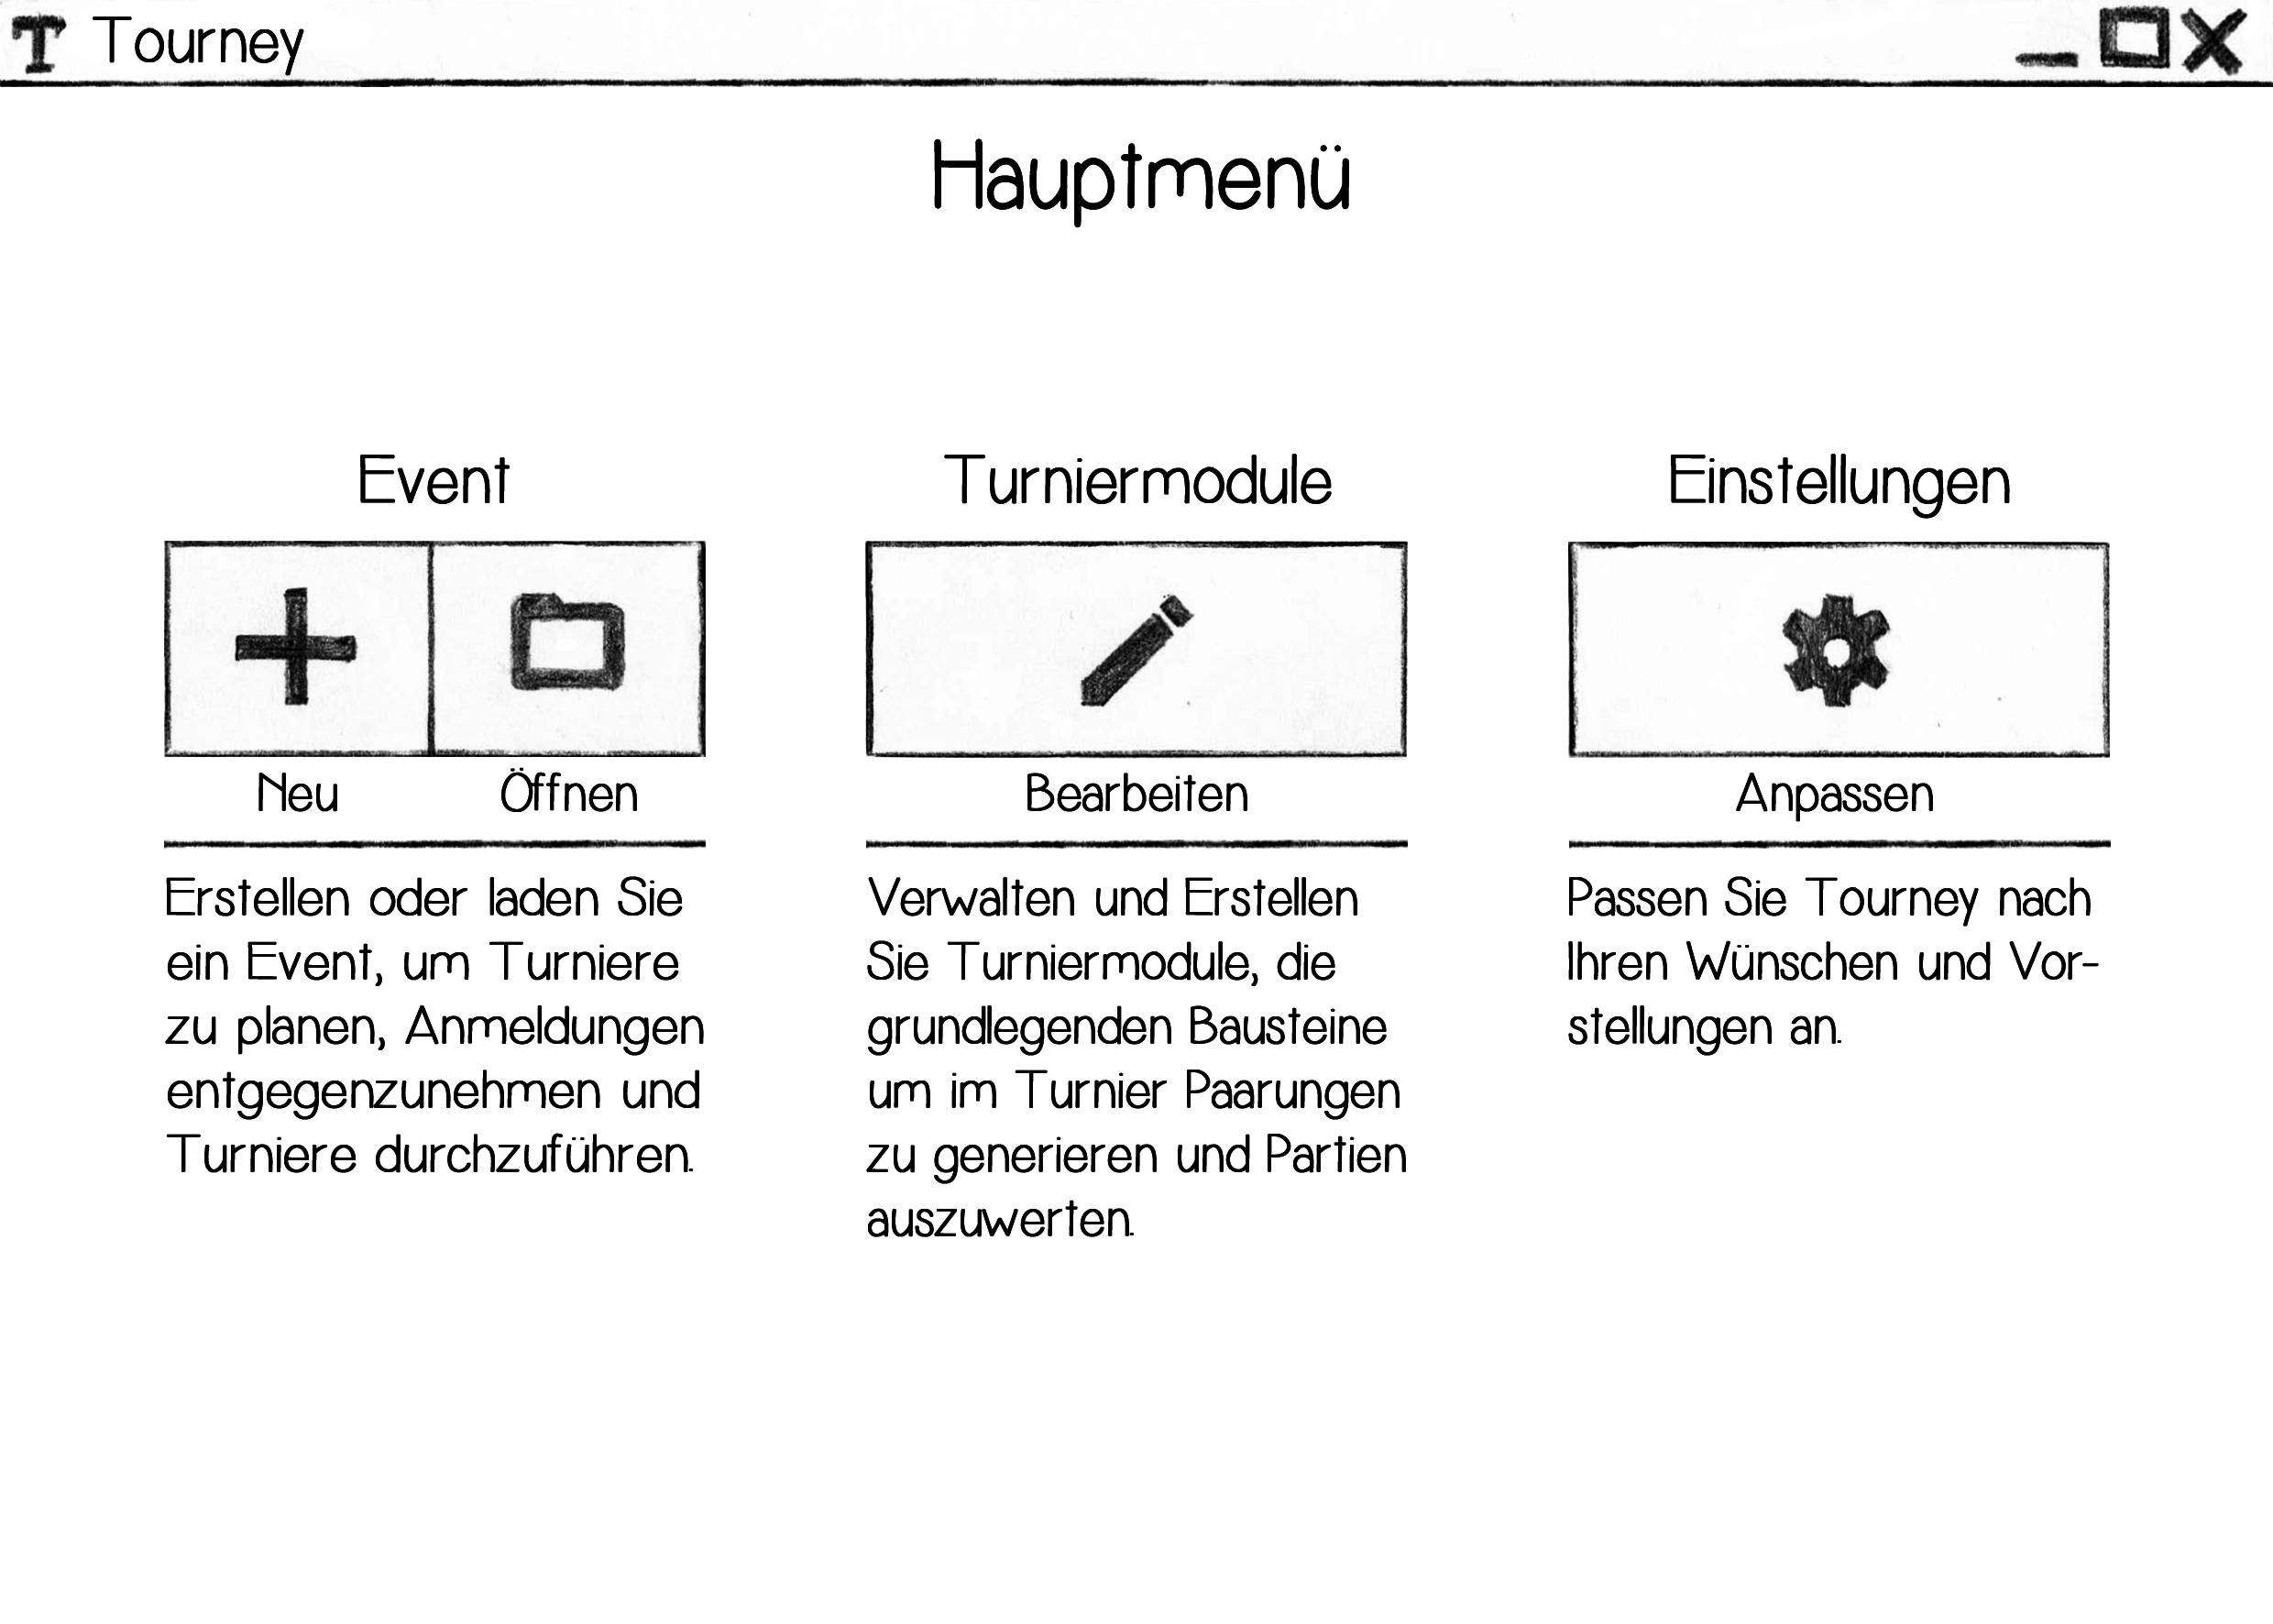
\includegraphics[width=\textwidth]{UIMockup/MainMenu.jpg}}

\vspace{1cm}

Im Hauptmenü hat der Nutzer die Möglichkeit zwischen verschiedenen Pfaden in der Benutzerführung zu wählen.

Entscheidet sich der Nutzer dazu, ein neues Event zu erstellen oder ein bestehendes zu öffnen springt die Software zur Darstellung der jeweils relevanten Projektphase.

Bei Betätigung des mittleren Knopfs erscheint eine veränderbare Auflistung aller bisher vorhandenen Regelmodule.

Will der Nutzer die Einstellung durch Betätigen des rechten Knopfs ändern öffnet sich das dafür vorgesehene Fenster.

\subsection{Einstellungen}

\fbox{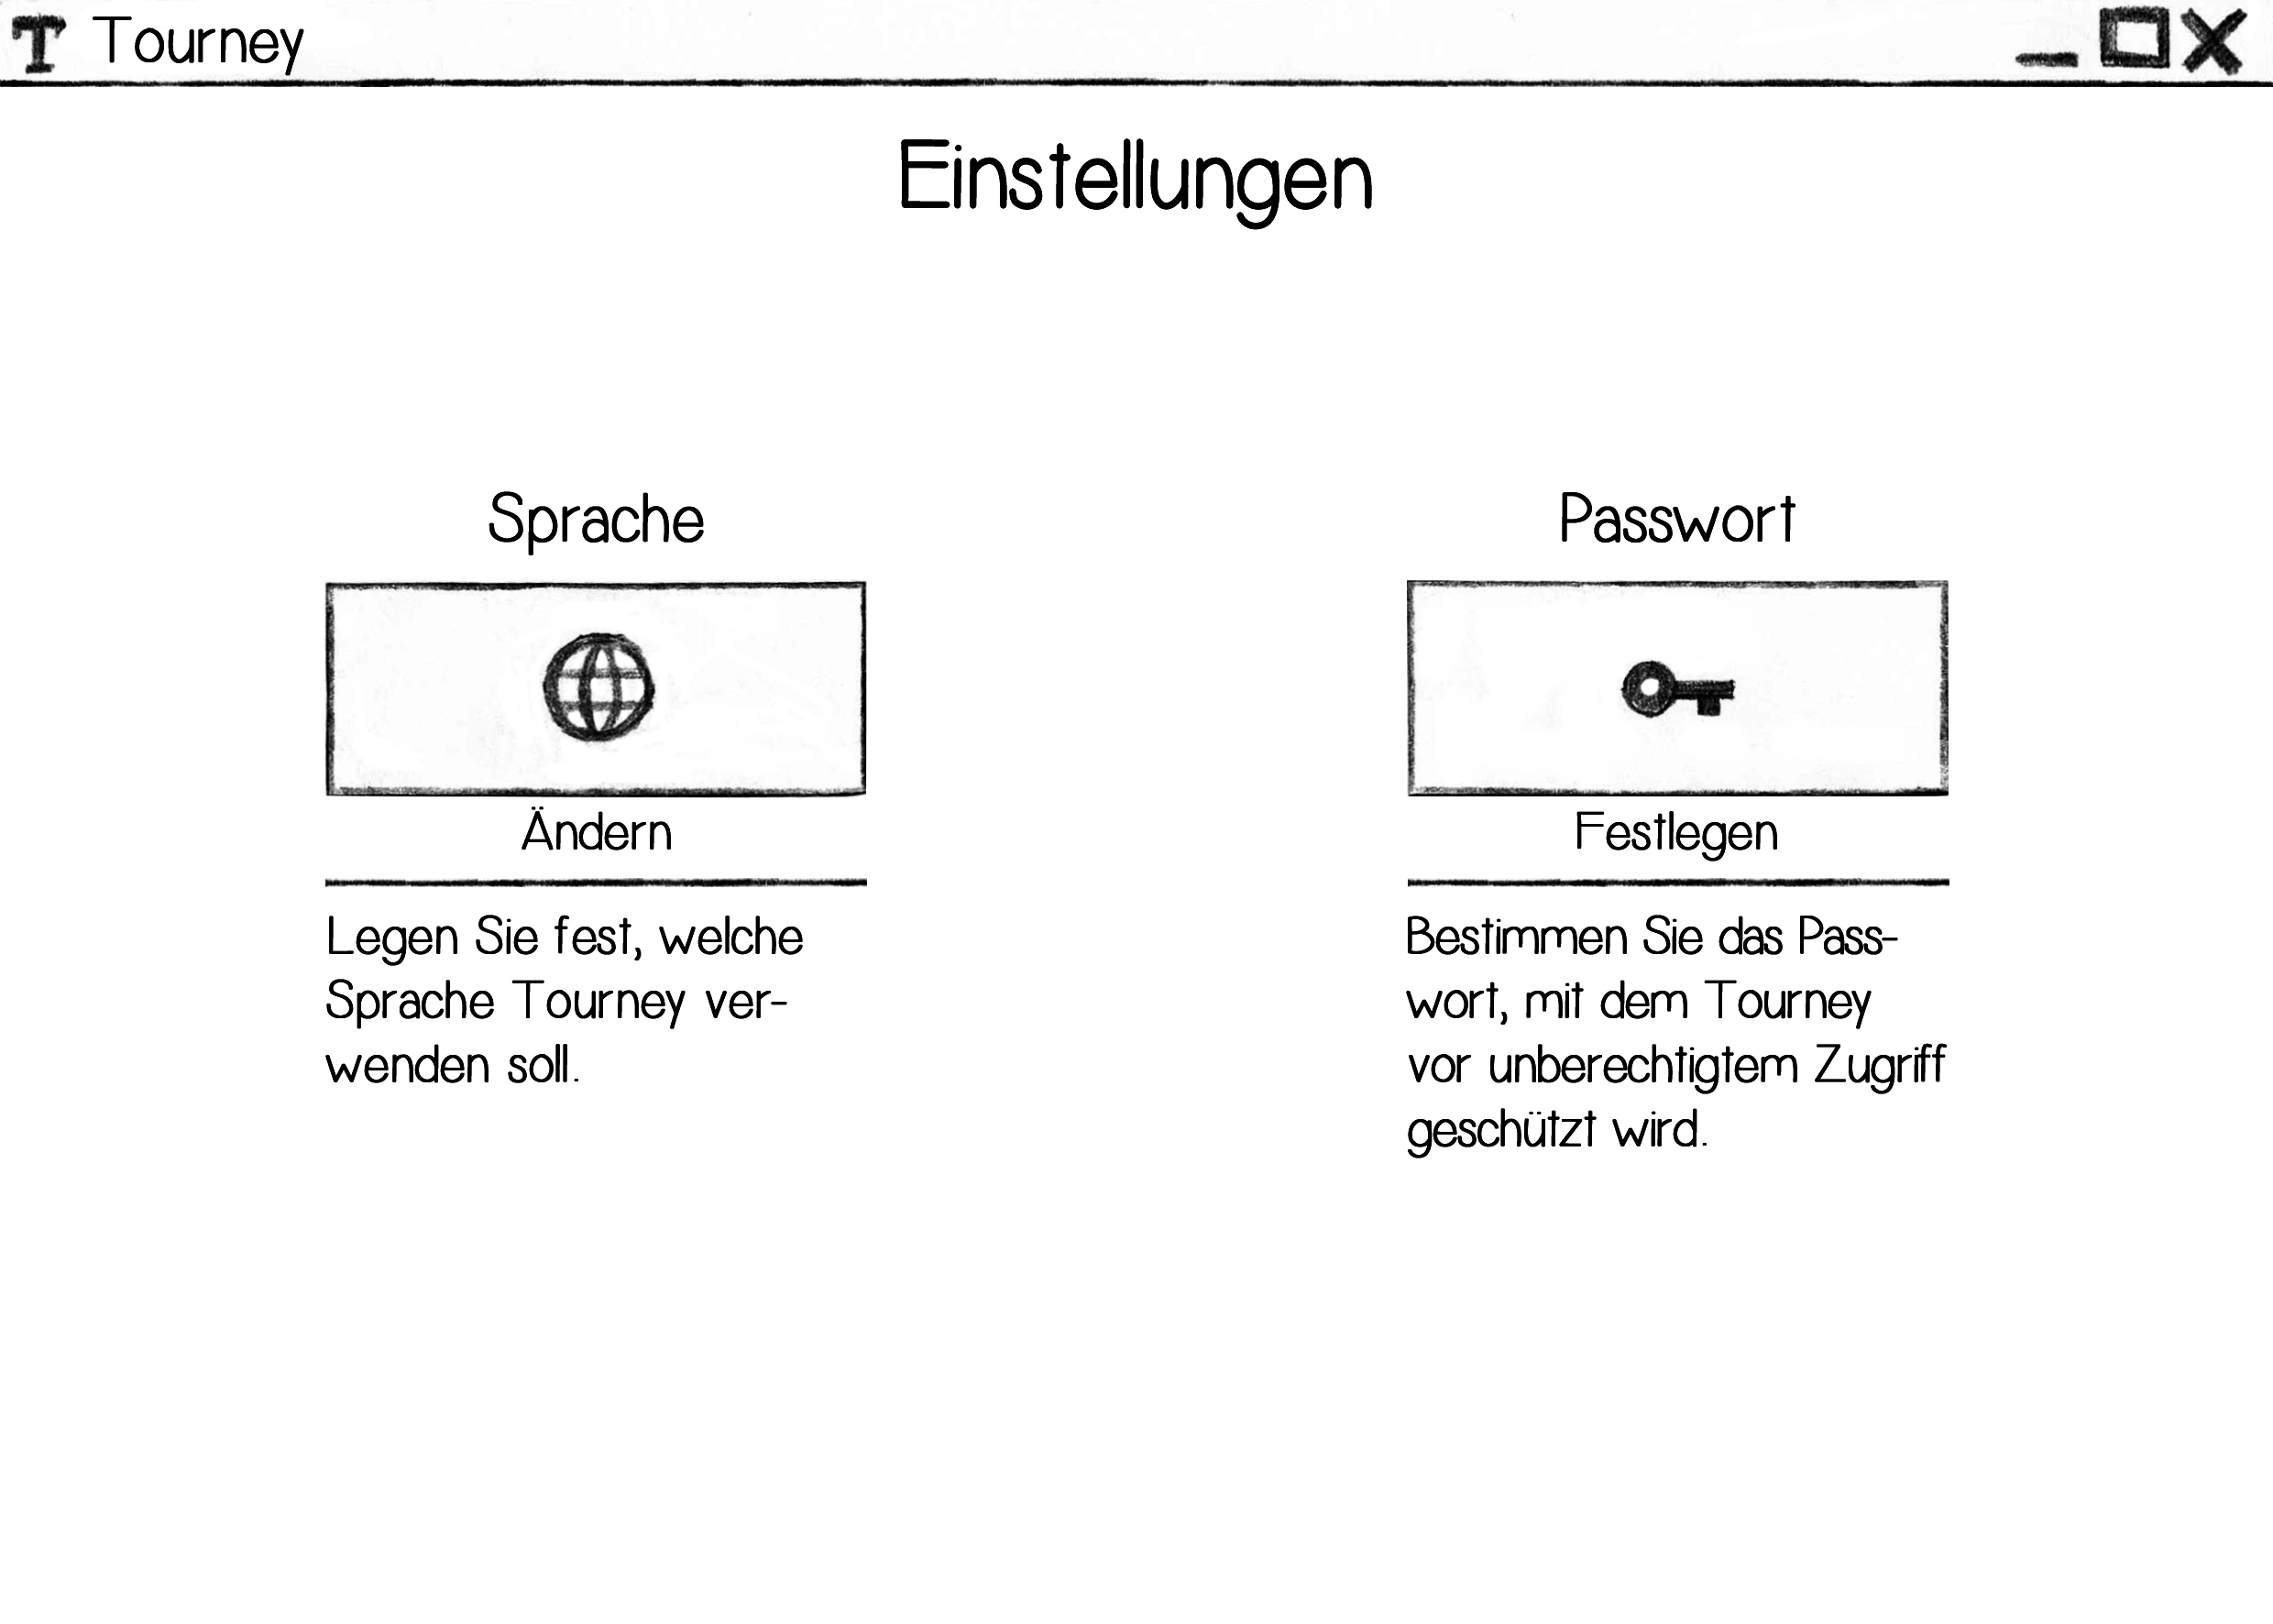
\includegraphics[width=\textwidth]{UIMockup/Settings.jpg}}

\vspace{1cm}

In den Einstellungen kann die verwendete Systemsprache aus einer Liste verfügbarer Sprachen(Deutsch/Englisch) ausgewählt und ein Passwort zur Sicherung des aktuellen Arbeitsplatzes festgelegt werden, dies ist beim ersten Start nicht gesetzt.

\subsection{Erstellung eines Events}

\fbox{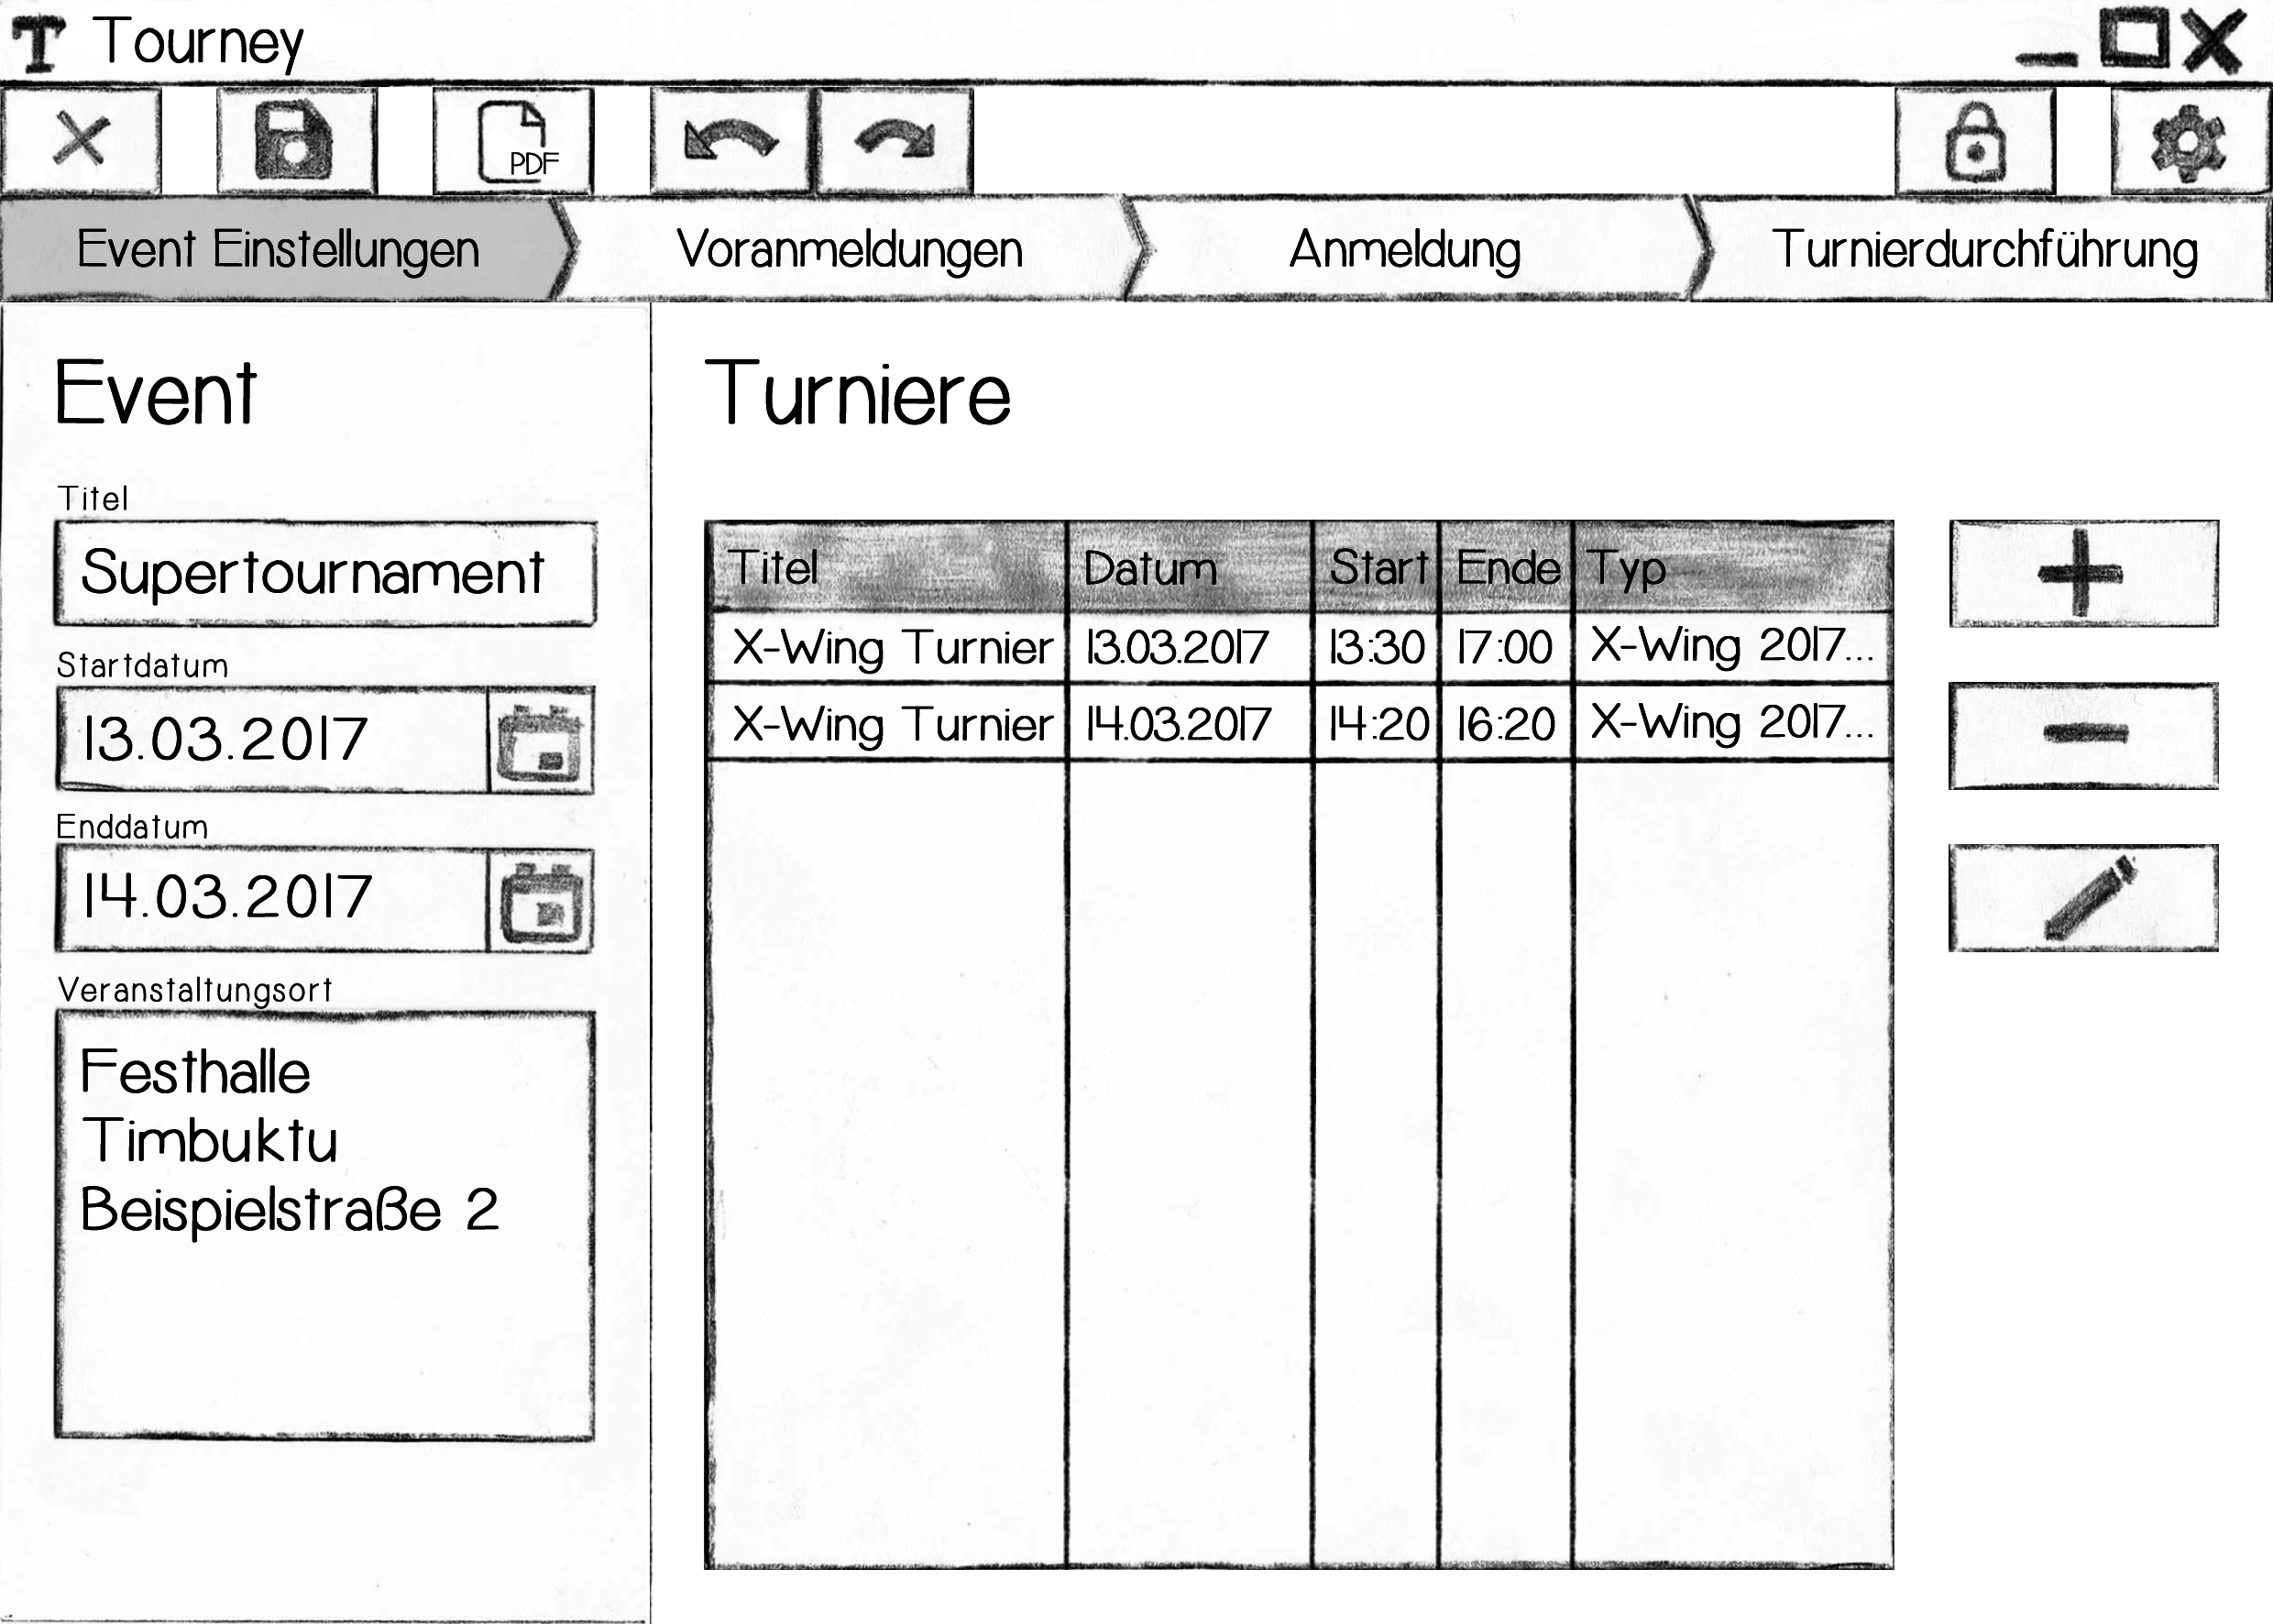
\includegraphics[width=\textwidth]{UIMockup/EventSetup.jpg}}

\vspace{1cm}

Die folgenden vier Fenster können erreicht werden, wenn ein neues Turnier erstellt oder ein vorhandenes bearbeitet oder durchgeführt werden soll. Die Fenster haben eine Reihe von Knöpfen am oberen Rand gemein, die von links nach rechts die folgenden Funktionen ausführen:
\newpage
\begin{itemize}
	\item Schließen des Fensters und Rückkehr zum Hauptmenü
	\item Speichern der Änderungen am aktuellen Event
	\item Rückgängig machen der letzten Eingabe
	\item Die letzte Änderung wiederherstellen
	\item Die Turnierergebnisse als PDF-Datei exportieren
	\item Daten für die kollaborative Anmeldung oder Turnierdurchführung exportieren
	\item Daten von anderen Arbeitsplätzen aus der Anmeldung oder Turnierdurchführung importieren und zusammenfügen
	\item Den benutzten Arbeitsplatz mit dem festgelegten Passwort sperren
	\item Die Einstellungen aufrufen
\end{itemize}
Zudem befindet sich unter diesen Knöpfen eine Leiste mit Projektphasen, die den Fortschritt in der Planung anzeigt und mit der zwischen den Phasen gewechselt werden kann.

In den allgemeinen Event-Einstellungen können mit den Bedienelementen links Titel, Veranstaltungsort und Zeitraum festgelegt werden, der aus einem Kalender ausgewählt werden kann.

Im rechten Teil des Fensters wird eine Liste aller hinzugefügten Turniere angezeigt, die durch die Knöpfe ganz rechts bearbeitet werden kann.

\subsection{Registrieren von Voranmeldungen}

\fbox{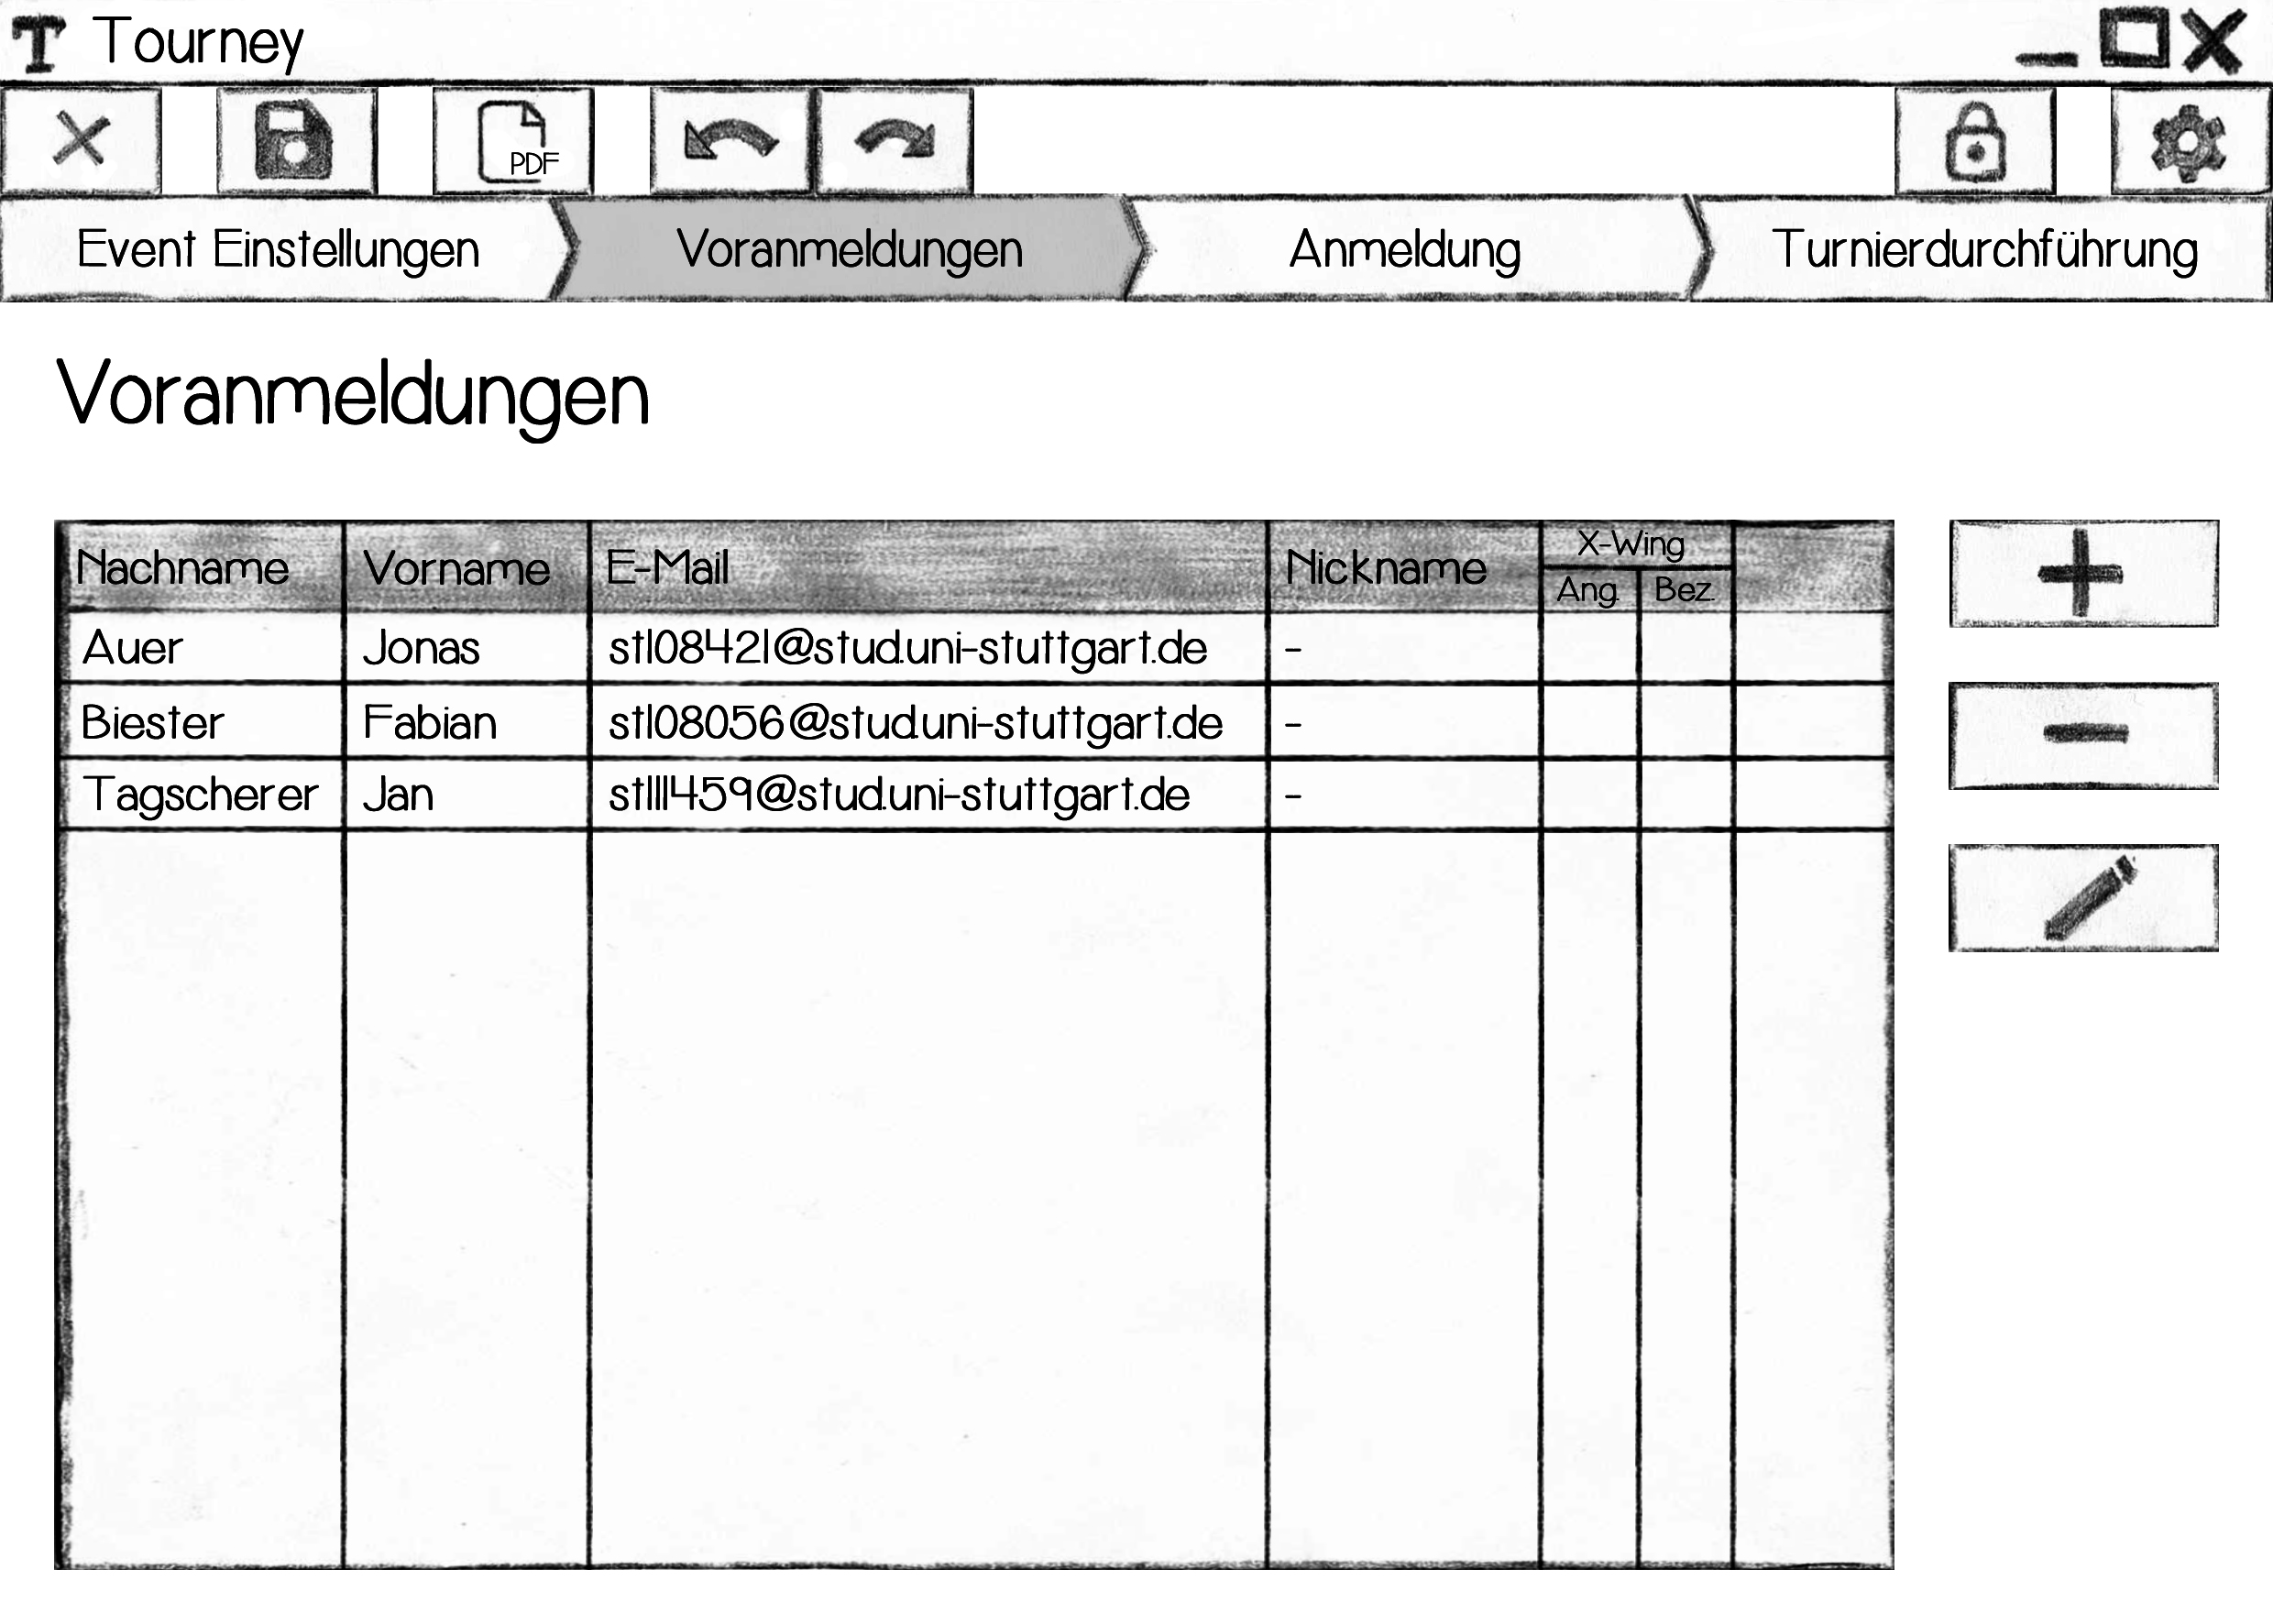
\includegraphics[width=\textwidth]{UIMockup/PreRegistration.jpg}}

\vspace{1cm}

Der Abschitt mit den Voranmeldungen bietet die Möglichkeit, eine Liste aller vorhandenen Voranmeldungen mit angemeldeten Turnieren und Bezahlstatus anzuzeigen und Einträge mit den Knöpfen rechts hinzuzufügen, zu löschen oder zu bearbeiten.

\subsection{Registrieren von Anmeldungen}

\fbox{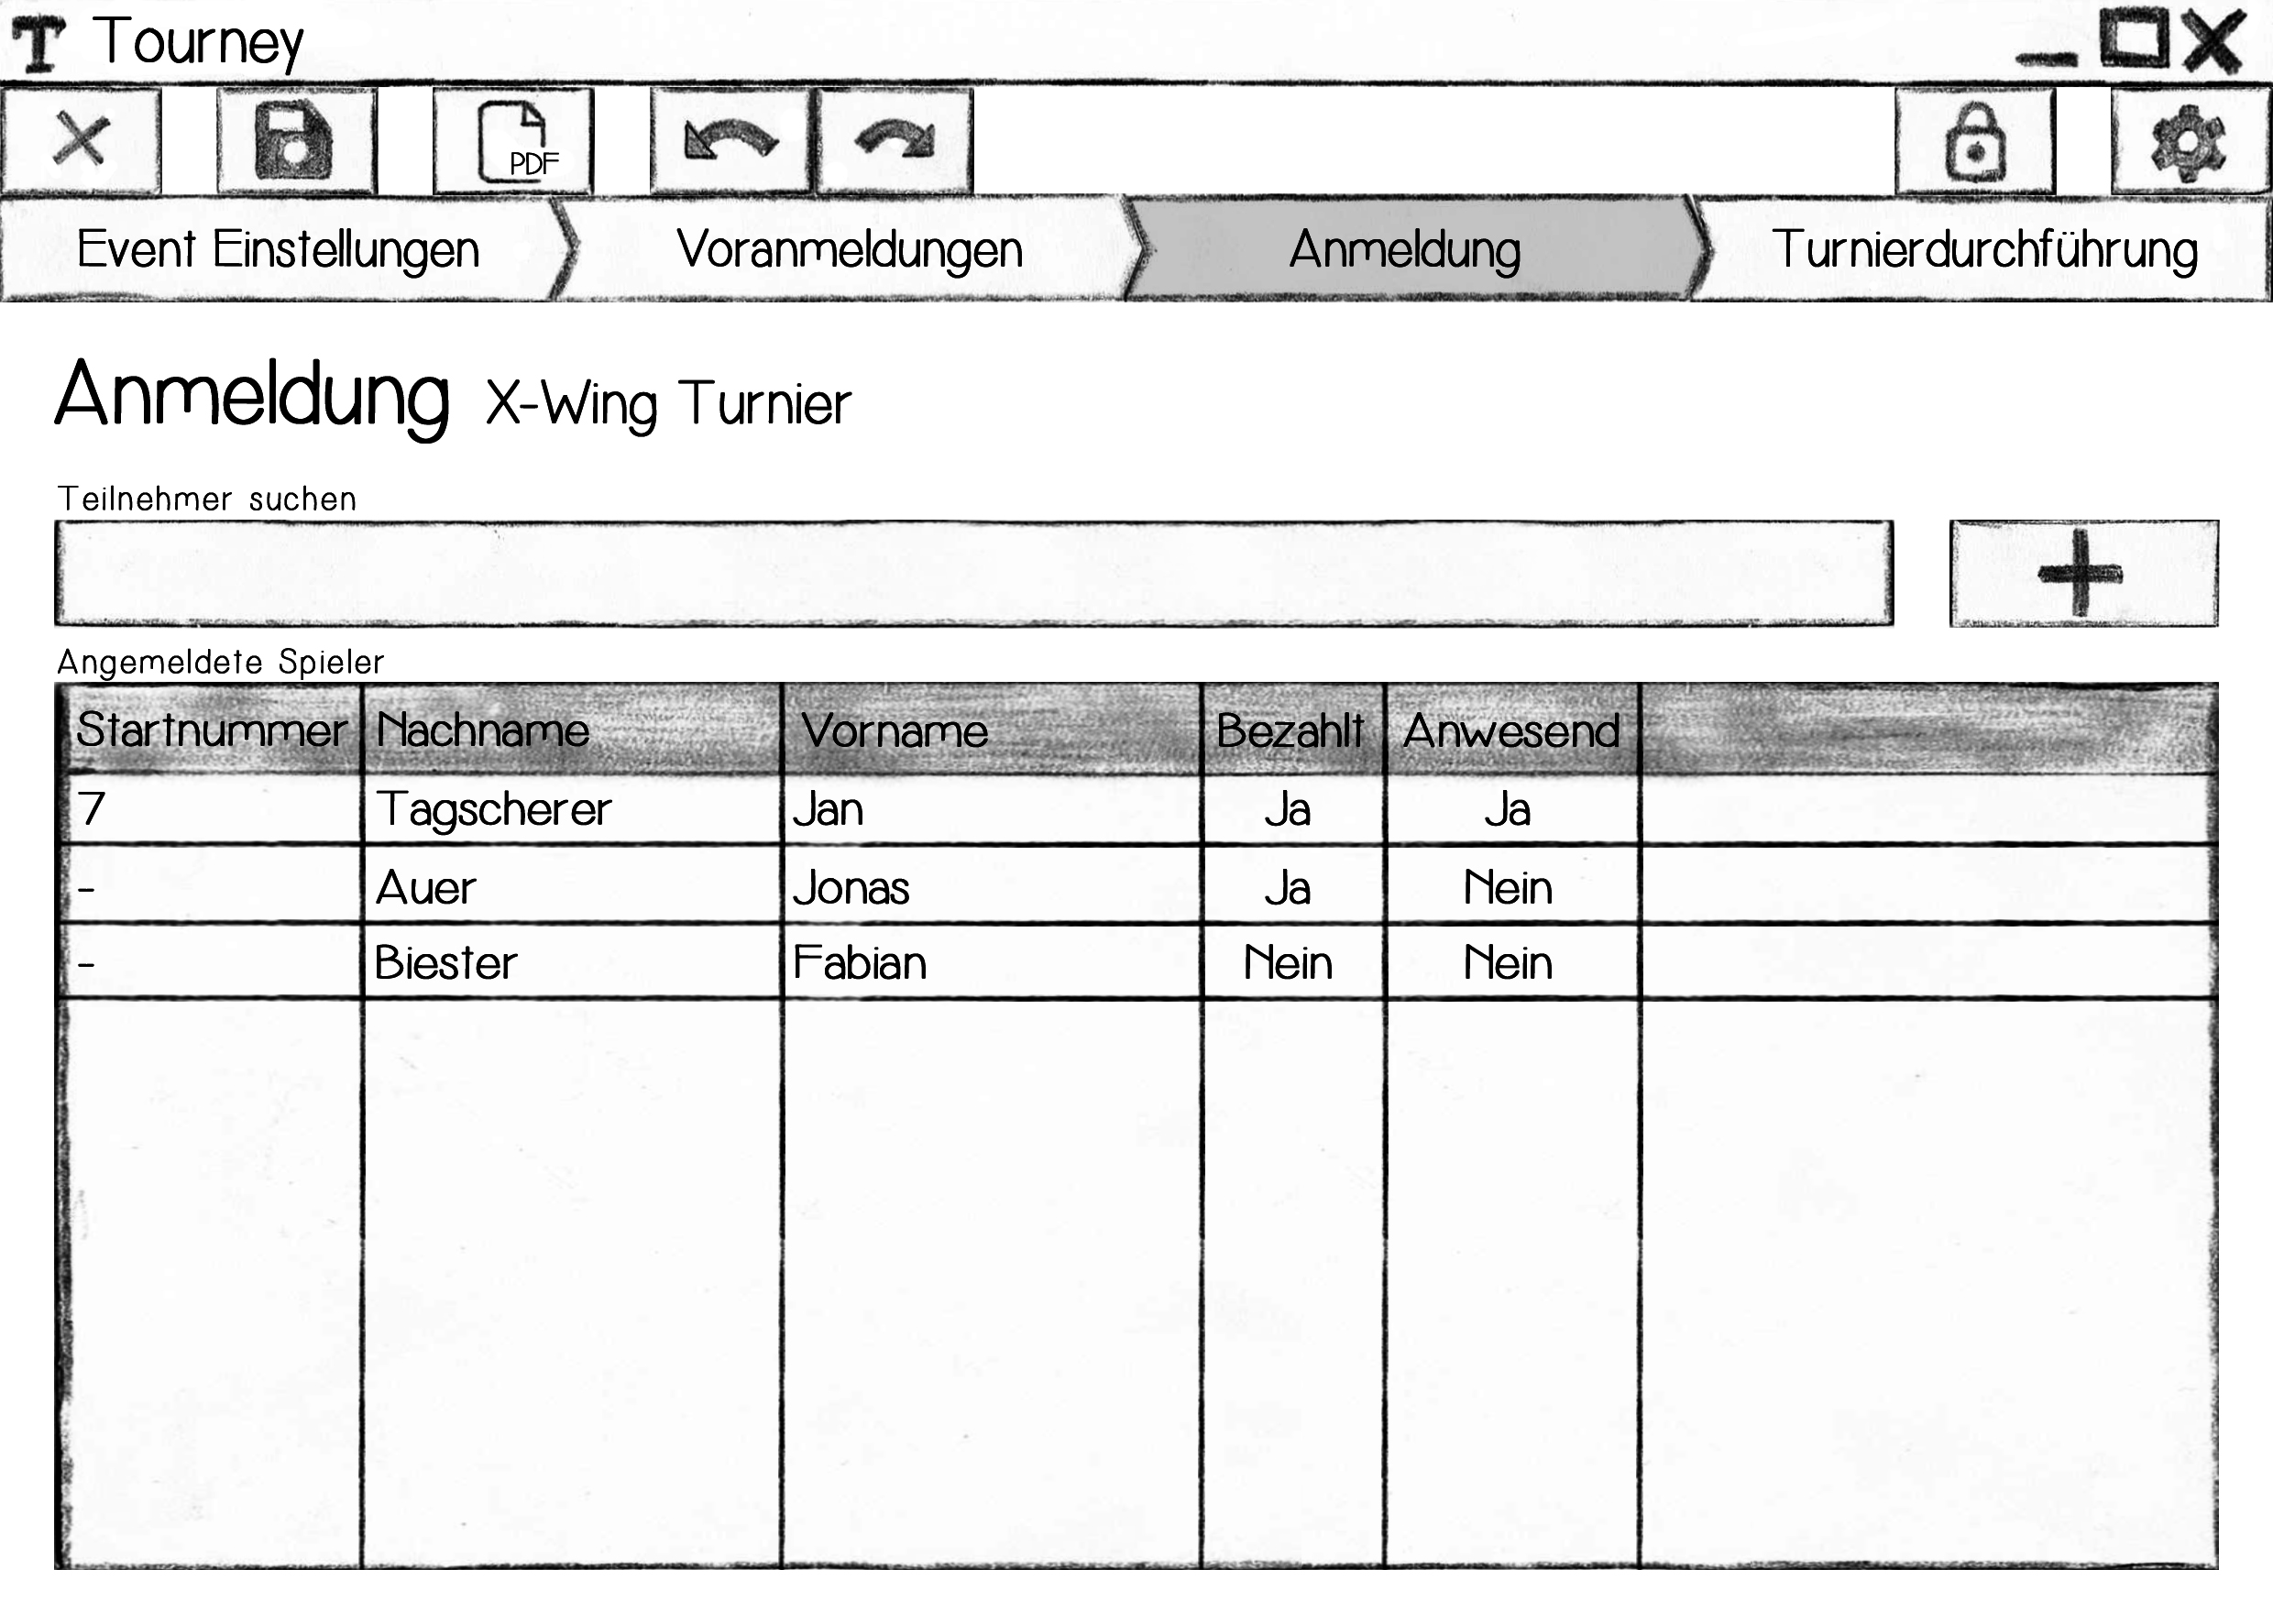
\includegraphics[width=\textwidth]{UIMockup/Registration.jpg}}

\vspace{1cm}

In der Anmeldungs-Phase können vorangemeldete Spieler mit den Bedienelementen in der oberen Hälfte gesucht und zu den angemeldeten Spielern hinzugefügt werden.

\subsection{Turnierdurchführung}

\fbox{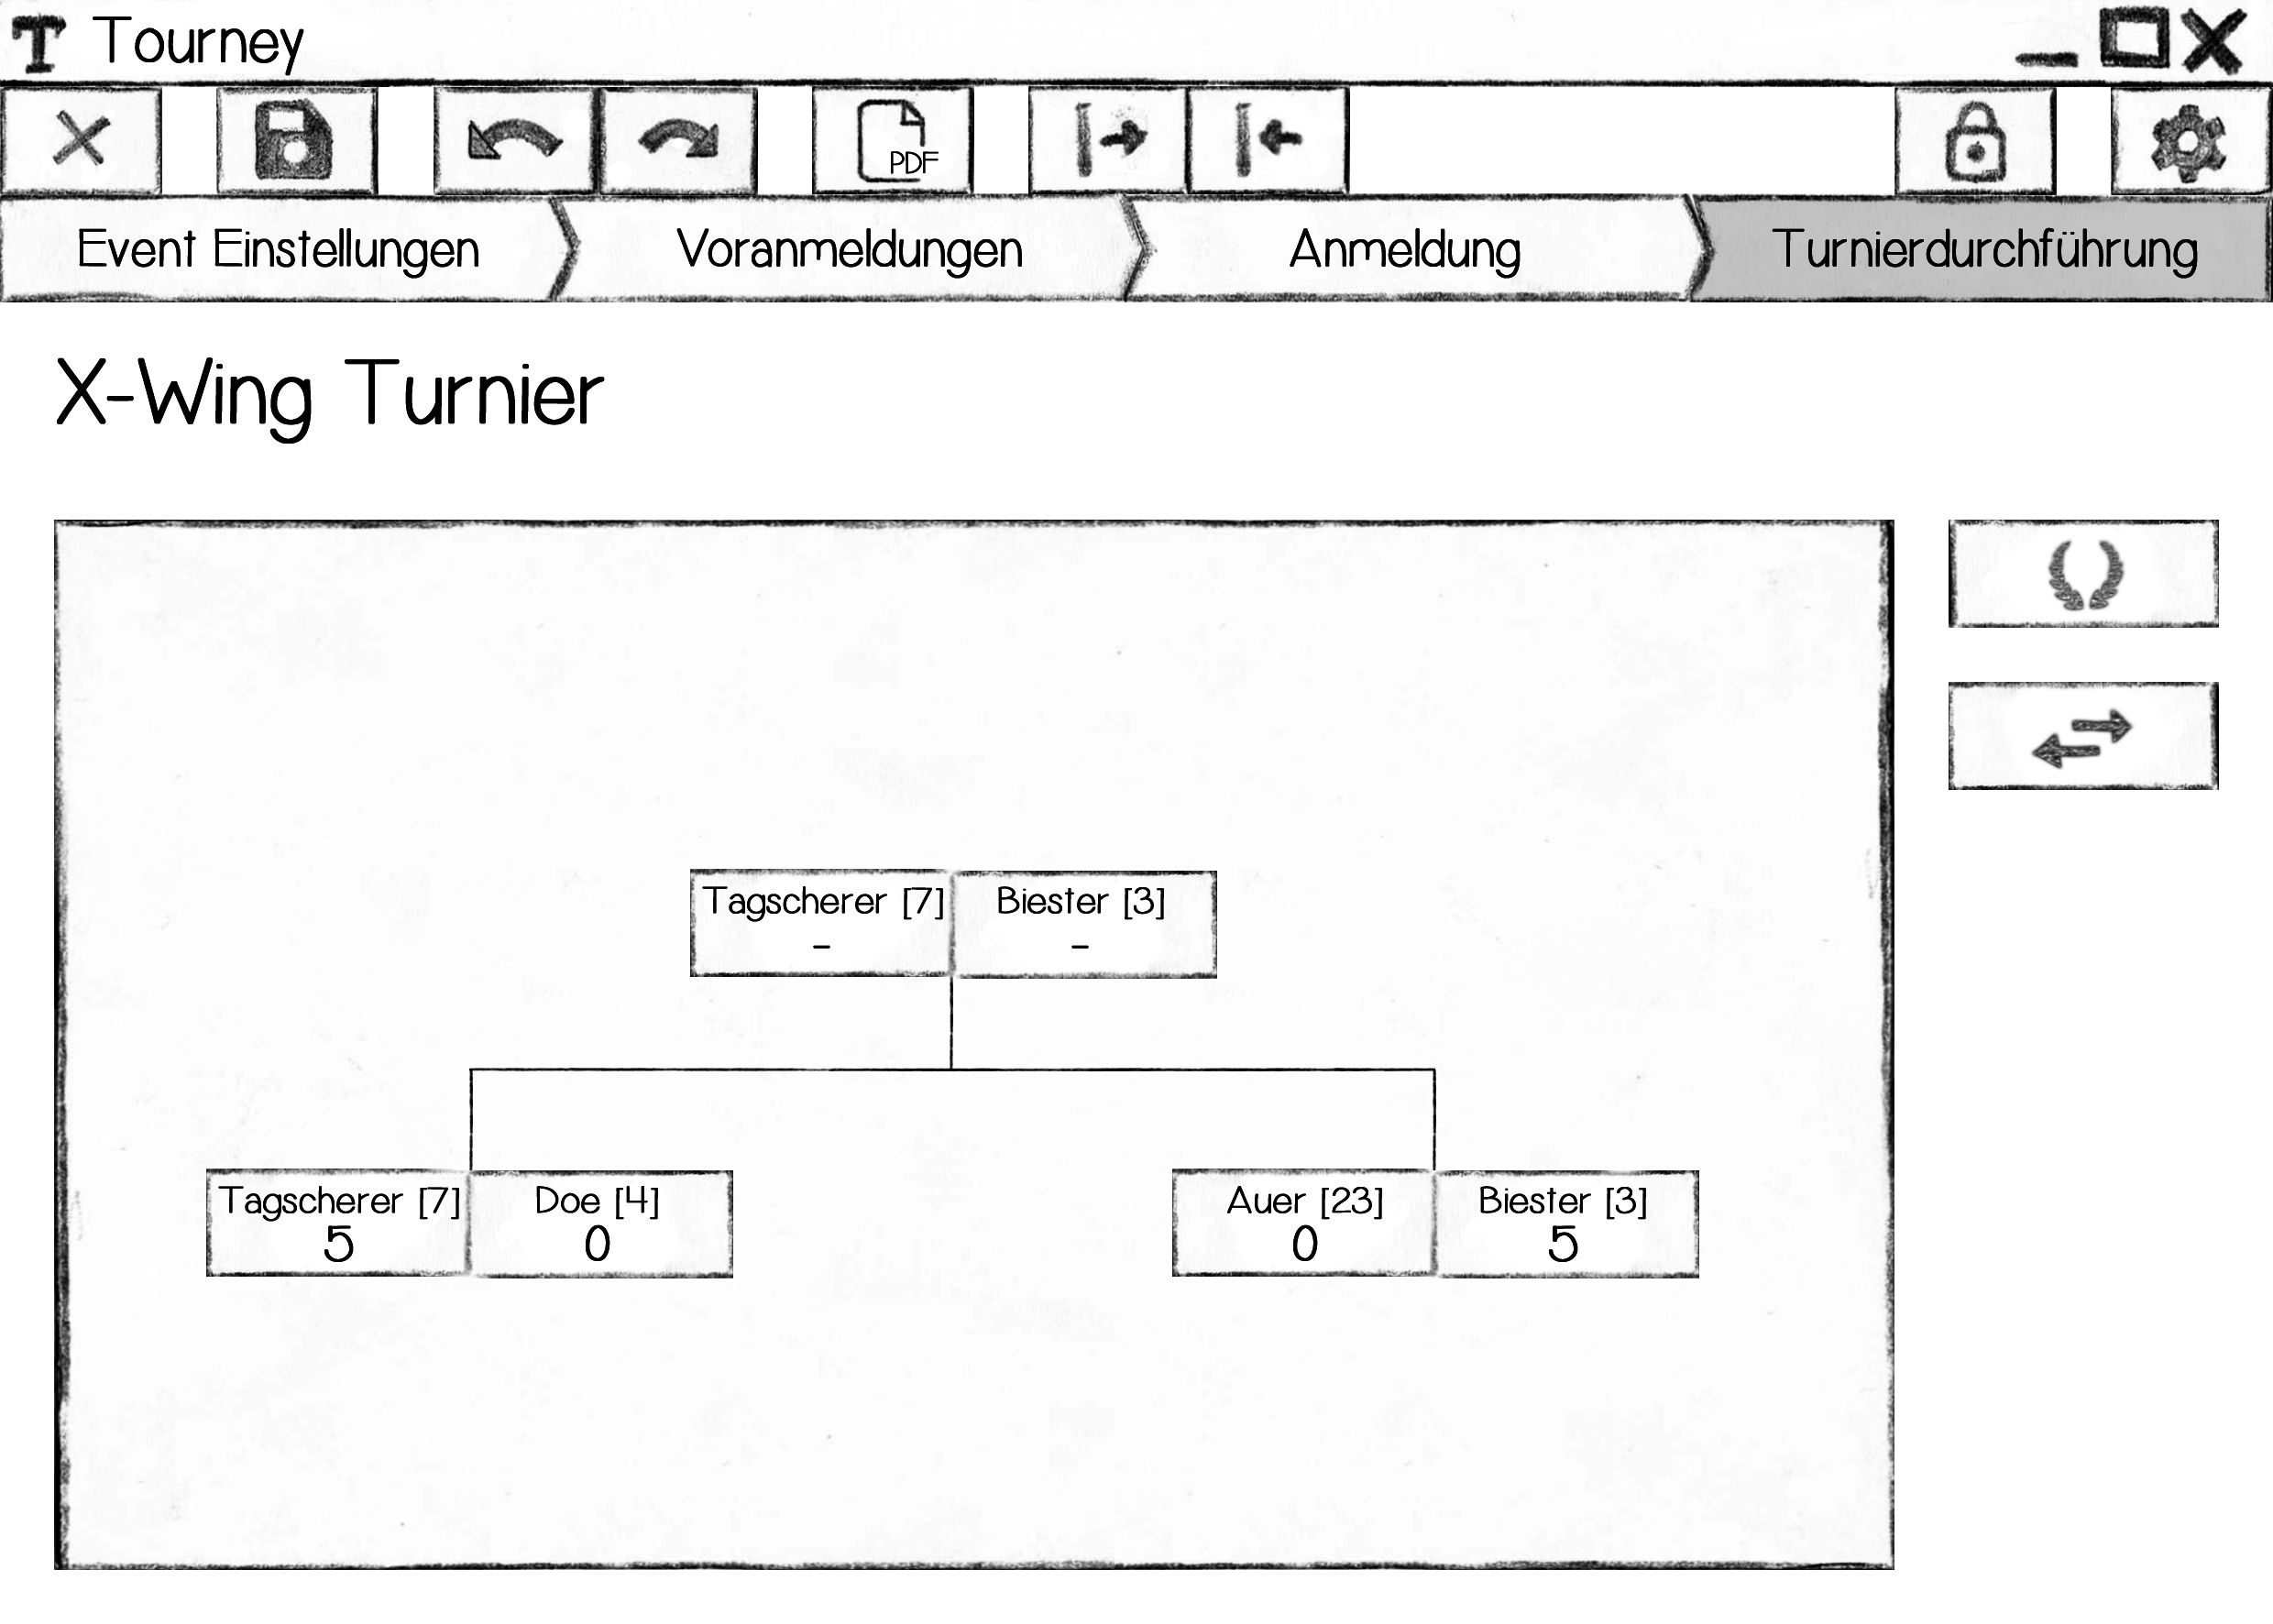
\includegraphics[width=\textwidth]{UIMockup/TournamentExecution.jpg}}

\vspace{1cm}

In der Durchführung eines einzelnen Turniers können stattfindende Paarungen angezeigt und diese mit den Knöpfen auf der rechten Seite verändert und Ergebnisse eingetragen werden.

\subsection{Erstellung von Turniermodulen}

\fbox{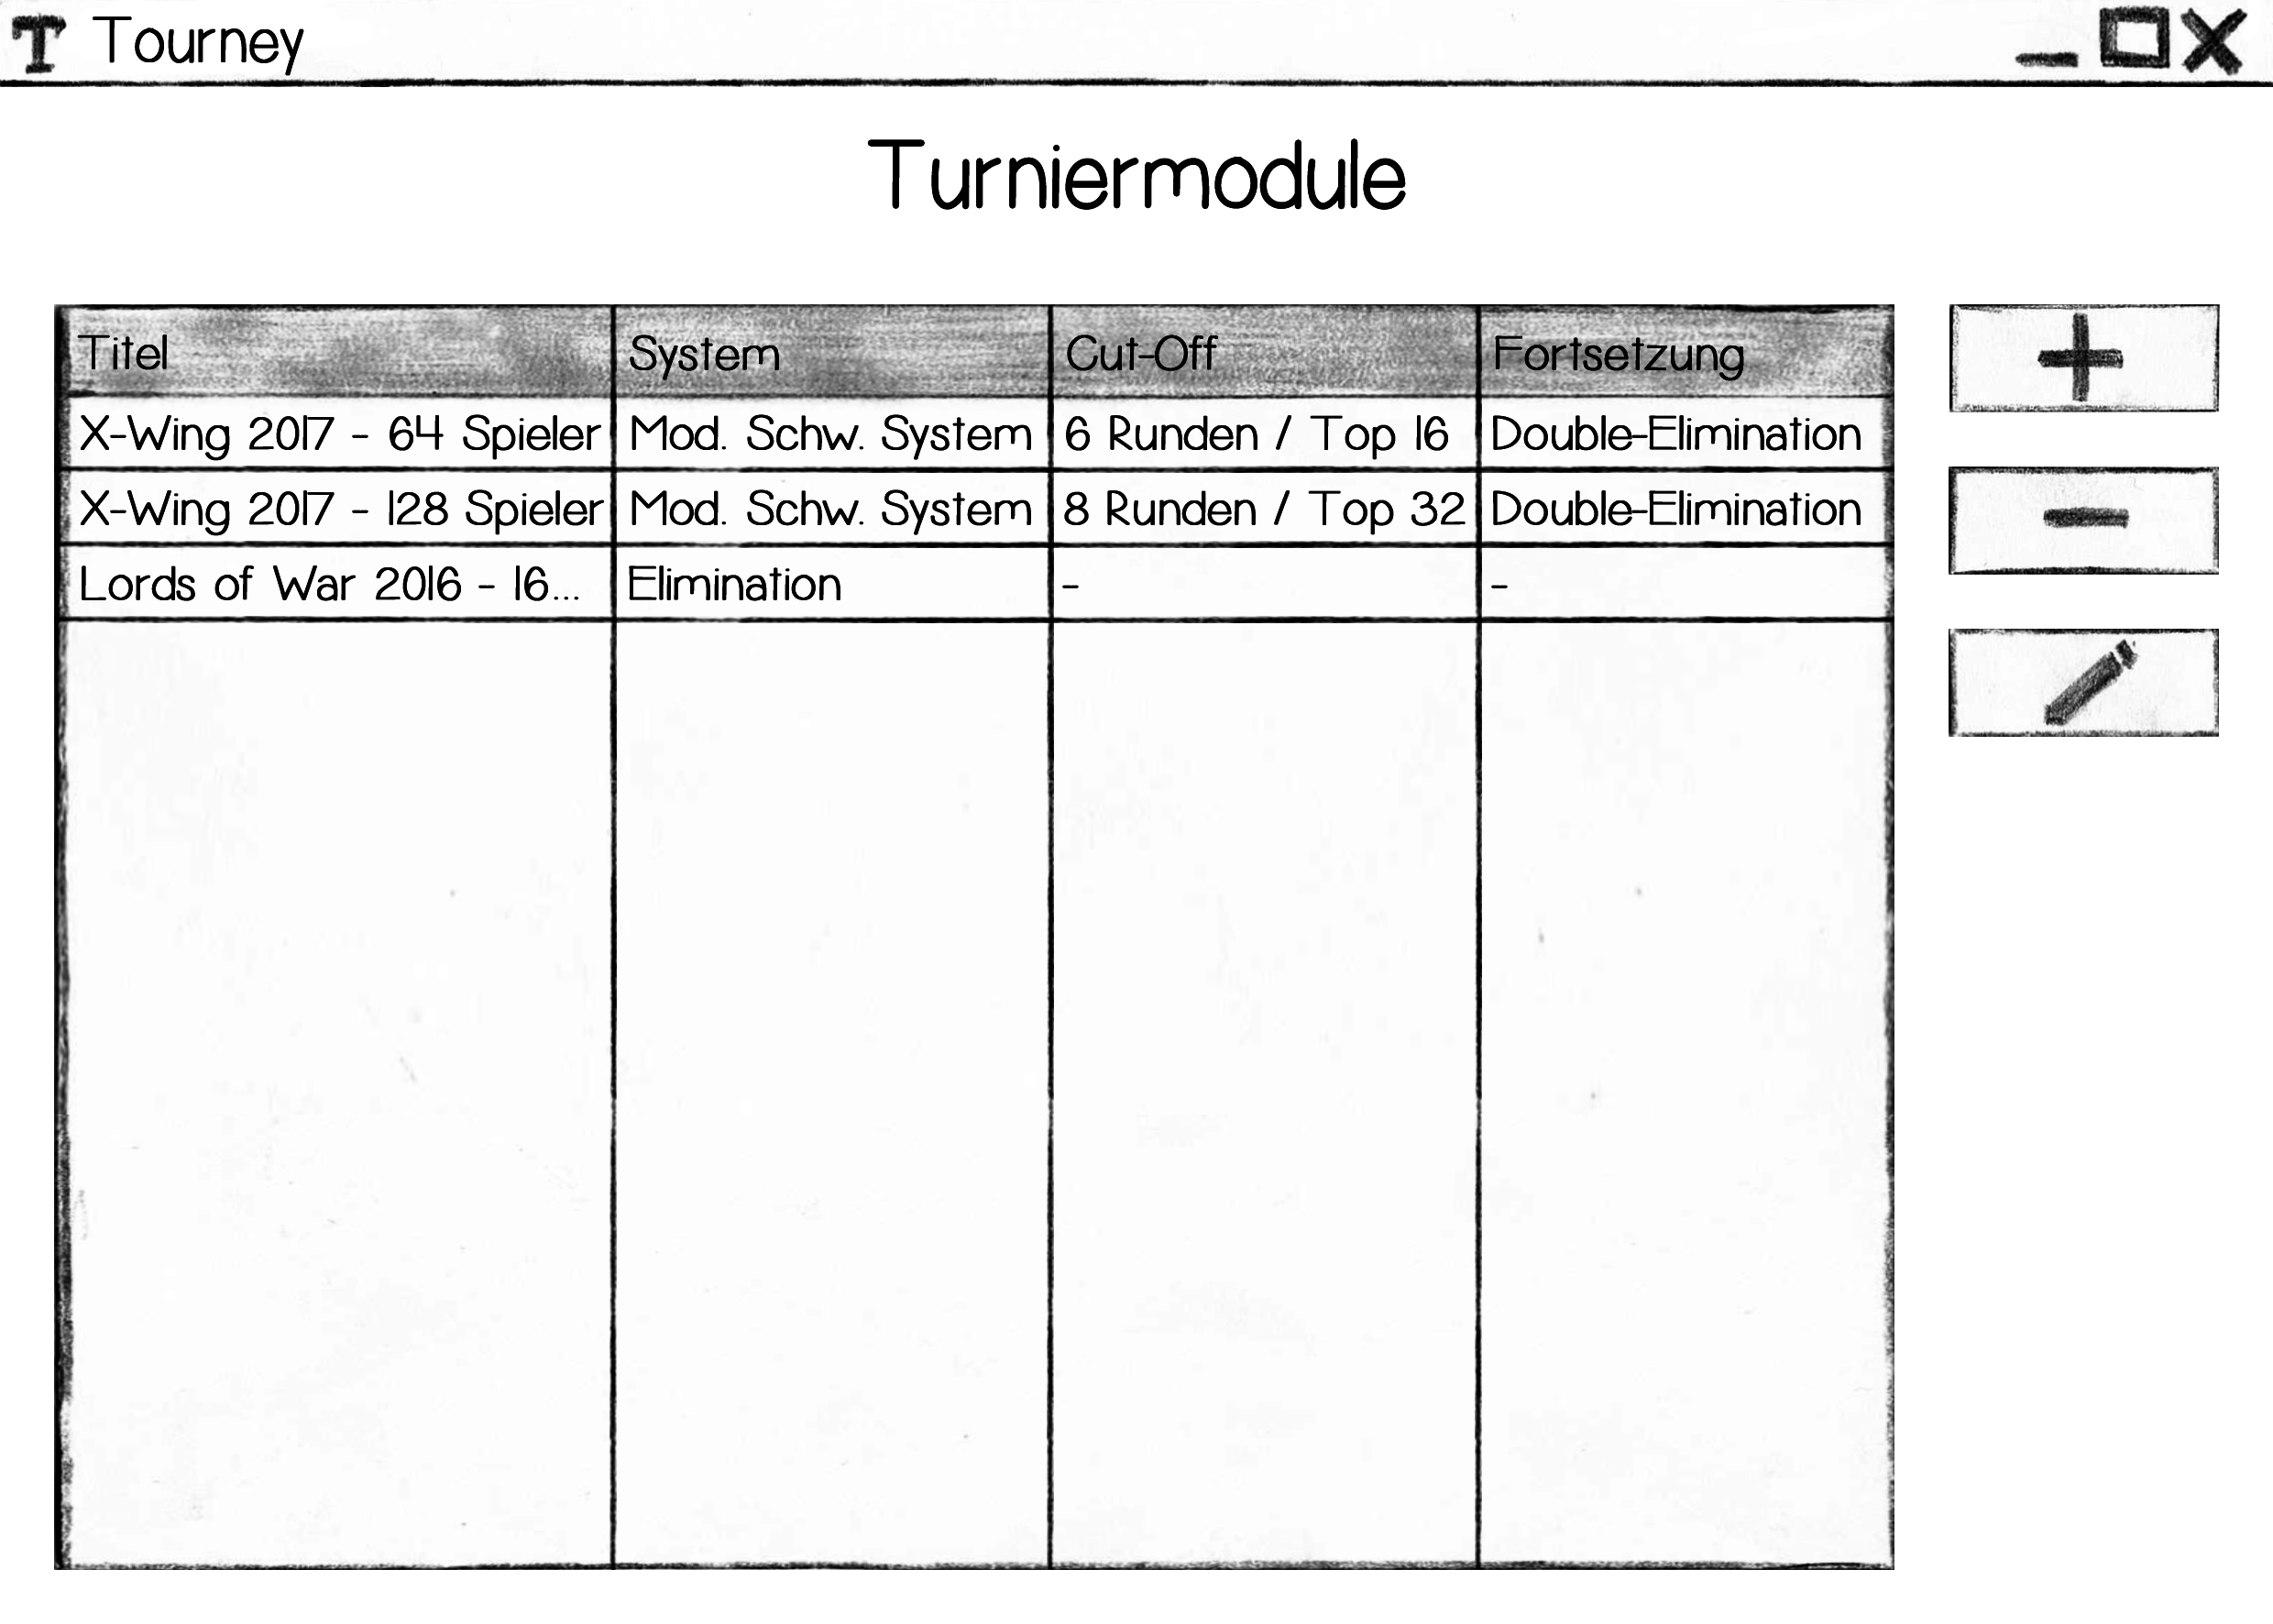
\includegraphics[width=\textwidth]{UIMockup/TournamentModulesList.jpg}}

\vspace{1cm}

Das Fenster mit den Turniermodulen gibt die Möglichkeit, eine Liste aller erstellten Regelmodule anzusehen und mit den Knöpfen auf der rechten Seite neue Einträge hinzuzufügen oder vorhandene zu löschen oder zu bearbeiten.

\section{Anwendungsfälle}

\subsection{Übersicht über die Anwendungsfälle}

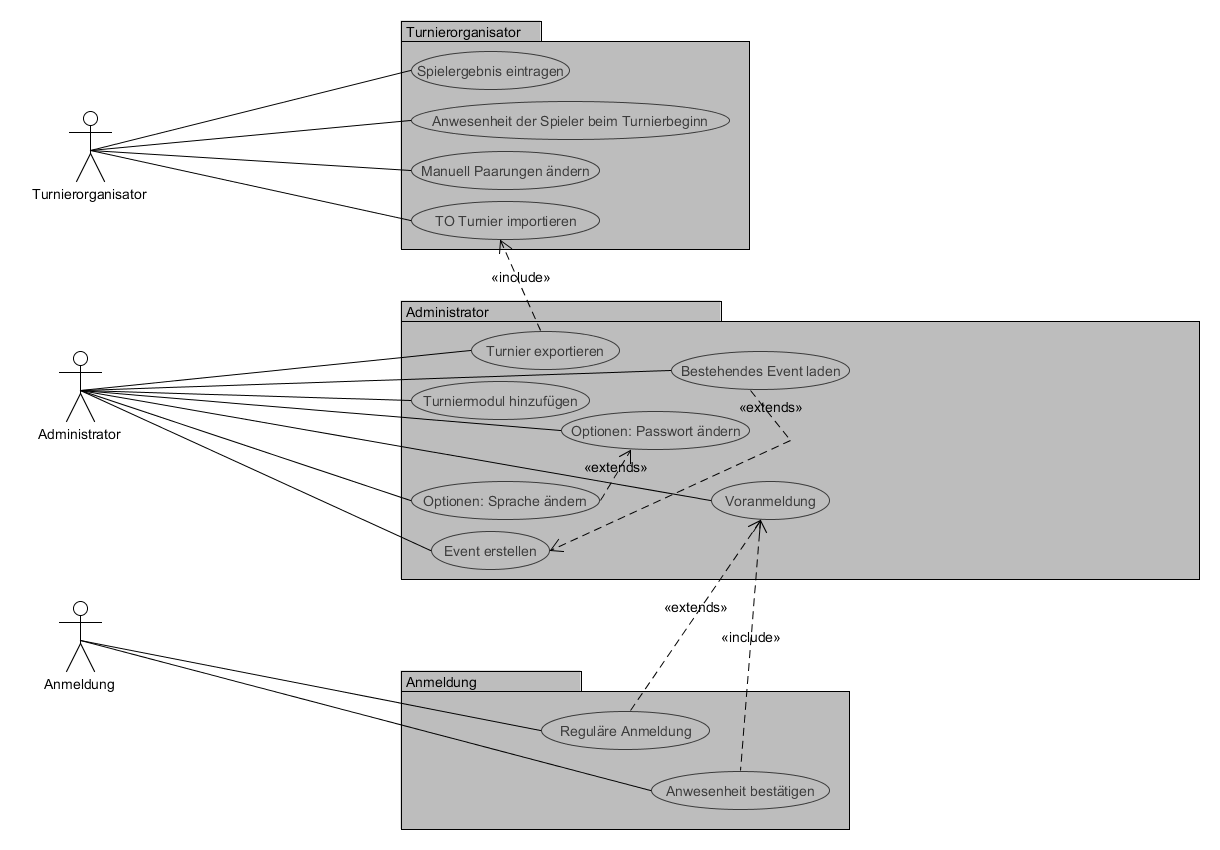
\includegraphics[width=\textwidth]{UseCaseDiagram.png}

\subsection{Anwendungsfälle des Administrators}

\subsubsection{Event erstellen}

\begin{tabularx}{\textwidth}{| p{0.2\textwidth} | p{0.7415\textwidth} |}
	\hline
	\textbf{ID} & 1 \\
	\hline
	\textbf{Ziel} & Es kann mit der Voranmeldung begonnen werden, daher ist das Event mit allen notwendigen Daten fertig erstellt \\
	\hline
	\textbf{Akteure} & Administrator \\
	\hline
	\textbf{Beschreibung} & Es wird das Event erstellt und mit den vorhanden Daten modifiziert \\
	\hline
	\textbf{Ebene} & Benutzersicht \\

	\hline
	\multicolumn{2}{| c |}{\textbf{Normalablauf}} \\
	\hline
	\textbf{Vorbedingung} & Anwendung wurde gestartet, Anwendung wurde falls nötig entsperrt \\
	\hline
	\textbf{Ablauf} &
		\begin{enumerate}
			\item[1.] Administrator: Beginnt das Erstellen eines neuen Events
			\item[2.] System: Öffnet den Dialog für das Erstellen der Events
			\item[3.] Administrator: Nutzer vergibt Startdatum, Enddatum, Titel und öffnet das Fenster um die Turniere hinzuzufügen
			\newline
			Sonderfall für Alternativablauf 3a: Standard-Module sind nicht vorhanden
			\item[4.] System: Erstellt Datenbank für Vorabanmeldung
			\item[5.] System: Öffnet Dialog um Speicherort des Event zu bestimmen
			\item[6.] Administrator: Nutzer wählt den Speicherort aus
			\item[7.] System: Speichert das Event an dem vogegebenen Ort
			\newline
			Sonderfall für Alternativablauf 7a: Ungenügende Berechtigung um in den Zielordner zu schreiben
		\end{enumerate}
	\\
	\hline
	\textbf{Nachbedingung} & Vorabanmeldung kann gestartet werden, Event wurde gespeichert \\
	\hline
	\multicolumn{2}{| c |}{\textbf{Alternativablauf 3a}} \\
	\hline
	\textbf{Vorbedingung} & Standard-Module sind nicht vorhanden \\
	\hline
	\textbf{Ablauf} &
		\begin{enumerate}
			\item[3a1.] System: Gibt eine Meldung aus, dass die Standard-Module nicht gefunden wurden und verweist auf das Erstellen eines neuen Turniermoduls
			\item[3a2.] Administrator: Erstellt ein Turniermodul (siehe Use Case 5: Turniermodul erstellen)
			\newline
			Sonderfall für Alternativablauf 3a2a: Schließt Dialog ohne ein neues Turniermodul zu erstellen
			\item[3a3.] Administrator: Der Nutzer fügt dieses daraufhin dem Event hinzu
		\end{enumerate}
	\\
	\hline
	\textbf{Nachbedingung} & Das Event enthält nun ein oder mehrere Turniere \\
	\hline
	\multicolumn{2}{| c |}{\textbf{Alternativablauf 3a2a}} \\
	\hline
	\textbf{Vorbedingung} & Schließt Dialog ohne ein neues Turniermodul zu erstellen \\
	\hline
	\textbf{Ablauf} &
		\begin{enumerate}
			\item[3a2a1.] System: Geht in Zustand Y über
		\end{enumerate}
	\\
	\hline
	\textbf{Nachbedingung} & Zustand Y \\
	\hline
	\multicolumn{2}{| c |}{\textbf{Alternativablauf 7a}} \\
	\hline
	\textbf{Vorbedingung} & Ungenügende Berechtigung um in den Zielordner zu schreiben \\
	\hline
	\textbf{Ablauf} &
		\begin{enumerate}
			\item[7a1.] System: Gibt eine Warnung aus, dass eine ungenügende Schreibberechtigung vorhanden ist
		\end{enumerate}
	\\
	\hline
	\textbf{Nachbedingung} & Nutzer wurde infomiert, dass er ein neues Speicherziel wählen muss oder seine Änderungen werden nicht gespeichert \\
	\hline
\end{tabularx}

\newpage

\subsubsection{Bestehendes Event laden}

\begin{tabularx}{\textwidth}{| p{0.2\textwidth} | p{0.7415\textwidth} |}
	\hline
	\textbf{ID} & 2 \\
	\hline
	\textbf{Ziel} & Bestehendes Event aus dem gespeicherten Zustand laden \\
	\hline
	\textbf{Akteure} & Administrator \\
	\hline
	\textbf{Beschreibung} & Lädt das gespeicherte Event inklusive Turniermodulen, Zuständen und Fortschritt im Turnier. Fragt gegebenenfalls ein gesetztes Passwort ab. \\
	\hline
	\textbf{Ebene} & Benutzersicht \\
	\hline
	\multicolumn{2}{| c |}{\textbf{Normalablauf}} \\
	\hline
	\textbf{Vorbedingung} & Programm ist gestartet, Anwendung ist entsperrt falls nötig \\
	\hline
	\textbf{Ablauf} &
		\begin{enumerate}
			\item[1.] Administrator: Will neues Event laden
			\item[2.] System: Öffnet den File Browser
			\item[3.] Administrator: Wählt die zu ladende Datei aus der Verzeichnisstruktur aus und bestätigt Auswahl
			\item[4.] System: Lädt den gespeicherten Zustand des Events
		\end{enumerate}
	\\
	\hline
	\textbf{Nachbedingung} & Der gespeicherte Zustand des Events ist geladen und benutzbar \\
	\hline
\end{tabularx}

\newpage

\subsubsection{Optionen (Sprache anzeigen und ändern)}

\begin{tabularx}{\textwidth}{| p{0.2\textwidth} | p{0.7415\textwidth} |}
	\hline
	\textbf{ID} & 3 \\
	\hline
	\textbf{Ziel} & Die aktuelle eingestellte Sprache anzeigen oder diese verändern. \\
	\hline
	\textbf{Akteure} & Administrator \\
	\hline
	\textbf{Beschreibung} & Der Nutzer möchte die eingestellte Sprache anzeigen oder aus den vorhandenen Sprachen eine andere auswählen. \\
	\hline
	\textbf{Ebene} & Benutzersicht \\
	\hline
	\multicolumn{2}{| c |}{\textbf{Normalablauf}} \\
	\hline
	\textbf{Vorbedingung} & Programm wurde gestartet \\
	\hline
	\textbf{Ablauf} &
		\begin{enumerate}
			\item[1.] Administrator: Öffnet die Optionen
			\item[2.] System: Öffnet das Optionen-Fenster, zeigt aktuelle Spracheinstellung an
			\item[3.] Administrator: Wählt andere Sprache (Englisch/Deutsch) aus
			\newline
			Sonderfall für Alternativablauf 3a: Will sich die Optionen nur anzeigen lassen und nicht verändern
			\newline
			Sonderfall für Alternativablauf 3b: Eingestellte Option ist dieselbe Sprache wie die aktuell ausgewählte
			\item[4.] System: Stellt die Sprache auf die ausgewählte Sprache um
		\end{enumerate}
	\\
	\hline
	\textbf{Nachbedingung} &  \\
	\hline
	\multicolumn{2}{| c |}{\textbf{Alternativablauf 3a}} \\
	\hline
	\textbf{Vorbedingung} & Will sich die Optionen nur anzeigen lassen und nicht verändern \\
	\hline
	\textbf{Ablauf} &
		\begin{enumerate}
			\item[3a1.] System: Es wird nichts verändert
			\item[3a2.] Administrator: Verlässt Optionen-Menü
		\end{enumerate}
	\\
	\hline
	\textbf{Nachbedingung} &  \\
	\hline
	\multicolumn{2}{| c |}{\textbf{Alternativablauf 3b}} \\
	\hline
	\textbf{Vorbedingung} & Eingestellte Option ist dieselbe Sprache wie die aktuell ausgewählte \\
	\hline
	\textbf{Ablauf} &
		\begin{enumerate}
			\item[3b1.] System: Belässt aktuelle Spracheinstellung
		\end{enumerate}
	\\
	\hline
	\textbf{Nachbedingung} & Programm wird in der eingestellten Sprache angezeigt \\
	\hline
\end{tabularx}

\subsubsection{Optionen (Passwort ändern)}

\begin{tabularx}{\textwidth}{| p{0.2\textwidth} | p{0.7415\textwidth} |}
	\hline
	\textbf{ID} & 4 \\
	\hline
	\textbf{Ziel} & Es soll ein neues Passwort gesetzt werden oder ein bestehendes geändert werden \\
	\hline
	\textbf{Akteure} & Administrator \\
	\hline
	\textbf{Beschreibung} & Der Nutzer möchte seine Anwendung mit einem Passwort sichern oder das 
          bestehende Passwort ändern \\
	\hline
	\textbf{Ebene} & Benutzersicht \\
	\hline
	\multicolumn{2}{| c |}{\textbf{Normalablauf}} \\
	\hline
	\textbf{Vorbedingung} & Anwendung ist gestartet, Anwendung ist falls nötig entsperrt \\
	\hline
	\textbf{Ablauf} &
		\begin{enumerate}
			\item[1.] Administrator: Will Optionen betrachten
			\item[2.] System: Öffnet Optionen-Fenster
			\item[3.] Administrator: Wählt Option aus, um das Passwort zu ändern
			\item[4.] System: Öffnet Dialog, in dem die Passwortänderung vollzogen wird
			\newline
			Sonderfall für Alternativablauf 4a: Es wurde noch kein Passwort gesetzt
			\item[5.] Administrator: Gibt altes Passwort falls vorhanden und danach zwei Mal das neue Passwort ein
			\item[6.] System: Ändert das Passwort um die Anwendung zu sperren
			\newline
			Sonderfall für Alternativablauf 6a: Nutzer hat kein neues Passwort eingegeben
		\end{enumerate}
	\\
	\hline
	\textbf{Nachbedingung} & Anwendung wird nach der Änderung mit dem neuen Passwort entsperrt \\
	\hline
	\multicolumn{2}{| c |}{\textbf{Alternativablauf 4a}} \\
	\hline
	\textbf{Vorbedingung} & Das aktuelle Passwort ist nicht vorhanden. \\
	\hline
	\textbf{Ablauf} &
		\begin{enumerate}
			\item[4a1.] System: Der Dialog enthält nur die Eingabemöglichkeiten für das neue Passwort und dessen Bestätigung
		\end{enumerate}
	\\
	\hline
	\textbf{Nachbedingung} & Das vom Nutzer gewählte Passwort wird nun zum entsperren benötigt. \\
	\hline
	\multicolumn{2}{| c |}{\textbf{Alternativablauf 6a}} \\
	\hline
	\textbf{Vorbedingung} & Nutzer hat kein neues Passwort eingegeben \\
	\hline
	\textbf{Ablauf} &
		\begin{enumerate}
			\item[6a1.] System: Das Passwort wird entfernt
		\end{enumerate}
	\\
	\hline
	\textbf{Nachbedingung} & Nutzer kann Anwendung nicht mehr sperren \\
	\hline
\end{tabularx}

\newpage

\subsubsection{Turniermodul hinzufügen}

\begin{tabularx}{\textwidth}{| p{0.2\textwidth} | p{0.7415\textwidth} |}
	\hline
	\textbf{ID} & 5 \\
	\hline
	\textbf{Ziel} & Der Nutzer will eine Turniervariante erstellen \\
	\hline
	\textbf{Akteure} & Administrator \\
	\hline
	\textbf{Beschreibung} & Es wird ein neues Turniermodul erstellt, das weitgehend frei modifizierbar ist und nachher als Vorlage für andere Events dienen kann \\
	\hline
	\textbf{Ebene} & Benutzersicht \\
	\hline
	\multicolumn{2}{| c |}{\textbf{Normalablauf}} \\
	\hline
	\textbf{Vorbedingung} & Tourney ist geöffnet, Der Nutzer befindet sich auf der Startseite oder beim Erstellen eines Events in der Phase, in der die Turniere hinzugefügt werden \\
	\hline
	\textbf{Ablauf} &
		\begin{enumerate}
			\item[1.] Administrator: Wählt aus, dass er eine neue Turniervorlage erstellen will
			\item[2.] System: Es öffnet sich ein Dialog, in dem der Nutzer die spezifischen Einstellungen für das Turnier vornehmen kann
			\item[3.] Administrator: Stellt die Einstellung ein und speichert die Änderungen
			\item[4.] System: Speichert die Einstellungen im Programmverzeichnis
			\newline
			Sonderfall für Alternativablauf 4a: Die Vorlage kann nicht gespeichert werden
		\end{enumerate}
	\\
	\hline
	\textbf{Nachbedingung} & Nutzer hat eine neue Vorlage für Turniere erstellt und kann diese in den Events verwenden \\
	\hline
	\multicolumn{2}{| c |}{\textbf{Alternativablauf 4a}} \\
	\hline
	\textbf{Vorbedingung} & Die Vorlage kann nicht gespeichert werden \\
	\hline
	\textbf{Ablauf} &
		\begin{enumerate}
			\item[4a1.] System: Zeigt eine Warnung an, dass die Änderungen nicht gespeichert werden können
		\end{enumerate}
	\\
	\hline
	\textbf{Nachbedingung} & Der Nutzer weiß, dass seine Änderung nicht gespeichert wurde \\
	\hline
\end{tabularx}

\newpage

\subsubsection{Voranmeldung von Spielern}

\begin{tabularx}{\textwidth}{| p{0.2\textwidth} | p{0.7415\textwidth} |}
	\hline
	\textbf{ID} & 6 \\
	\hline
	\textbf{Ziel} & Voranmeldungen vor dem Event erfassen und speichern \\
	\hline
	\textbf{Akteure} & Administrator \\
	\hline
	\textbf{Beschreibung} & Der Nutzer hat von mindestens einem Spieler Voranmeldungen erhalten und möchte diese in das Event eintragen \\
	\hline
	\textbf{Ebene} & Benutzersicht \\
	\hline
	\multicolumn{2}{| c |}{\textbf{Normalablauf}} \\
	\hline
	\textbf{Vorbedingung} & Anwendung wurde gestartet, Der Nutzer hat ein Event erstellt und befindet sich in der Phase Voranmeldung, Die Anwendung ist entsperrt, Der übermittelte Datensatz ist vollständig \\
	\hline
	\textbf{Ablauf} &
		\begin{enumerate}
			\item[1.] Administrator: Wählt Option aus, um einen neuen Spieler hinzuzufügen
			\item[2.] System: Öffnet die Eingabemaske um die Daten einzutragen
			\item[3.] Administrator: Trägt den Teilnehmer in die Maske ein (Name, Vorname, Turniere an denen er teilnehmen möchte und optional E-Mail-Adresse)
			\item[4.] System: Überprüft, ob alle Angaben korrekt sind und trägt diese in die Datenbank ein
			\newline
			Sonderfall für Alternativablauf 4a: Getätigte Eingabe ist inkorrekt
		\end{enumerate}
	\\
	\hline
	\textbf{Nachbedingung} & Teilnehmer ist in Datenbank eingetragen \\
	\hline
	\multicolumn{2}{| c |}{\textbf{Alternativablauf 4a}} \\
	\hline
	\textbf{Vorbedingung} & Getätigte Eingabe ist inkorrekt \\
	\hline
	\textbf{Ablauf} &
		\begin{enumerate}
			\item[4a1.] System: Gibt eine Fehlermeldung aus und lässt den Nutzer die Eingaben nochmal überprüfen und verändern
		\end{enumerate}
	\\
	\hline
	\textbf{Nachbedingung} & Eingabe ist korrekt \\
	\hline
\end{tabularx}

\newpage

\subsubsection{Reguläre Anmeldung von Spielern}

\begin{tabularx}{\textwidth}{| p{0.2\textwidth} | p{0.7415\textwidth} |}
	\hline
	\textbf{ID} & 7 \\
	\hline
	\textbf{Ziel} & Der Spieler soll in die Datenbank eingetragen und für die einzelnen Turniere registriert sein \\
	\hline
	\textbf{Akteure} & Anmeldung (Hauptakteur) \\
	\hline
	\textbf{Beschreibung} & Spieler meldet sich bei der Anmeldung für verschiedene Turniere an. Dies wird dann in die Datenbank geschrieben \\
	\hline
	\textbf{Ebene} & Benutzersicht \\
	\hline
	\multicolumn{2}{| c |}{\textbf{Normalablauf}} \\
	\hline
	\textbf{Vorbedingung} & Anwendung wurde gestartet, Der Administrator hat ein Event erstellt, Die Anmeldung hat dieses Event importiert, Anwendung ist entsperrt, Das Event befindet sich in der Phase Anmeldung \\
	\hline
	\textbf{Ablauf} &
		\begin{enumerate}
			\item[1.] Spieler: Gibt der Anmeldung die erforderlichen Daten zum Anmelden
			\item[2.] Anmeldung: Gibt Daten in dafür vorgesehene Maske ein
			\item[3.] System: Trägt die Daten in die Datenbank ein
		\end{enumerate}
	\\
	\hline
	\textbf{Nachbedingung} & Spieler befindet sich in der Event-Datenbank \\
	\hline
\end{tabularx}

\newpage

\subsubsection{Anwesenheit eines vorangemeldeten Spielers bestätigen}

\begin{tabularx}{\textwidth}{| p{0.2\textwidth} | p{0.7415\textwidth} |}
	\hline
	\textbf{ID} & 8 \\
	\hline
	\textbf{Ziel} & Die Anwesenheit der vorangemeldeten Spieler bestätigen und den Bezahlstatus der Gebühr registrieren \\
	\hline
	\textbf{Akteure} & Anmeldung (Hauptakteur) \\
	\hline
	\textbf{Beschreibung} & Der vorangemeldete Spieler gibt seinen Namen und seine E-Mail-Adresse der Anmeldung. Diese sucht daraufhin in der Datenbank nach dem Namen und bestätigt, dass dieser anwesend ist und bezahlt hat \\
	\hline
	\textbf{Ebene} & Benutzersicht \\
	\hline
	\multicolumn{2}{| c |}{\textbf{Normalablauf}} \\
	\hline
	\textbf{Vorbedingung} & Anwendung muss gestartet sein, Anwendung muss entsperrt sein, Das Event muss erstellt worden sein, Das Event muss sich in der Phase 'Anmeldung' befinden, Das Event muss von der Anmeldung importiert worden sein, Spieler muss in der Datenbank enthalten sein \\
	\hline
	\textbf{Ablauf} &
		\begin{enumerate}
			\item[1.] Spieler: Gibt der Anmeldung Name und E-Mail-Adresse
			\item[2.] Anmeldung: Wählt Option, um die Voranmeldung zu verifizieren
			\item[3.] System: Öffnet die Maske, in der Name und E-Mail-Adresse eingegeben werden können
			\item[4.] Anmeldung: Gibt Name und E-Mail-Adresse ein, bestätigt gegebenenfalls Anwesenheit und Bezahlstatus und gibt Auftrag zur Verifikation
			\item[5.] System: Ändert Datenbankeintrag des Spielers und fügt ihn dem Turnier/den Turnieren hinzu
		\end{enumerate}
	\\
	\hline
	\textbf{Nachbedingung} & Spieler ist verifiziert und den Turnieren hinzugefügt \\
	\hline
\end{tabularx}

\newpage

\subsubsection{Turnier exportieren}

\begin{tabularx}{\textwidth}{| p{0.2\textwidth} | p{0.7415\textwidth} |}
	\hline
	\textbf{ID} & 9 \\
	\hline
	\textbf{Ziel} & Turnier ist als Datei exportiert \\
	\hline
	\textbf{Akteure} & Administrator \\
	\hline
	\textbf{Beschreibung} & Das Turnier soll an den Turnierorganisator weitergegeben werden, dieser kann das einzelne Turnier importieren \\
	\hline
	\textbf{Ebene} & Benutzersicht \\
	\hline
	\multicolumn{2}{| c |}{\textbf{Normalablauf}} \\
	\hline
	\textbf{Vorbedingung} & Anwendung muss gestartet sein, Anwendung muss entsperrt sein, Ein Event muss erstellt sein, Das Event muss in der Phase 'Turniere exportieren' sein. \\
	\hline
	\textbf{Ablauf} &
		\begin{enumerate}
			\item[1.] Administrator: Wählt Option, um Turniere zu exportieren
			\item[2.] System: Öffnet das Fenster zum Auswählen des Speicherorts für das exportierte Turnier
			\item[3.] Administrator: Exportiert das Turnier
		\end{enumerate}
	\\
	\hline
	\textbf{Nachbedingung} & Turnier muss exportiert sein \\
	\hline
\end{tabularx}

\newpage

\subsection{Anwendungsfälle der Turnierordner}

\subsubsection{Turnier importieren}

\begin{tabularx}{\textwidth}{| p{0.2\textwidth} | p{0.7415\textwidth} |}
	\hline
	\textbf{ID} & 10 \\
	\hline
	\textbf{Ziel} & Das Turnier soll importiert sein \\
	\hline
	\textbf{Akteure} & Turnierordner \\
	\hline
	\textbf{Beschreibung} & Der Turnierordner bekommt die Datei des Turniers und importiert dieses \\
	\hline
	\textbf{Ebene} & Benutzersicht \\
	\hline
	\multicolumn{2}{| c |}{\textbf{Normalablauf}} \\
	\hline
	\textbf{Vorbedingung} & Die Anwendung muss gestartet sein, Die Anwendung muss entsperrt sein, Das exportierte Turniermodul muss vorhanden sein, Nutzer muss auf der Startseite sein \\
	\hline
	\textbf{Ablauf} &
		\begin{enumerate}
			\item[1.] Turnierordner: Wählt Option um ein Turnier zu importieren
			\item[2.] System: Öffnet den File Browser um das Turnier zu importieren
			\item[3.] Turnierordner: Wählt die exportierte Turnier-Datei aus
			\item[4.] System: Importiert das Turnier
		\end{enumerate}
	\\
	\hline
	\textbf{Nachbedingung} & Das Turnier muss importiert sein \\
	\hline
\end{tabularx}

\newpage

\subsubsection{Anwesenheit der Spieler bei Turnierbeginn feststellen}

\begin{tabularx}{\textwidth}{| p{0.2\textwidth} | p{0.7415\textwidth} |}
	\hline
	\textbf{ID} & 11 \\
	\hline
	\textbf{Ziel} & Anwesenheit der Spieler beim Turnierbeginn feststellen \\
	\hline
	\textbf{Akteure} & Turnierordner \\
	\hline
	\textbf{Beschreibung} & Der Turnierordner überprüft die Anwesenheit der einzelnen Spieler, damit die Paarungen bestimmt werden können \\
	\hline
	\textbf{Ebene} & Benutzersicht \\
	\hline
	\multicolumn{2}{| c |}{\textbf{Normalablauf}} \\
	\hline
	\textbf{Vorbedingung} & Anwendung muss gestartet sein, Anwendung muss entsperrt sein, Turnier muss geladen sein, Turnier muss in der Phase 'Anwesenheit kontrollieren' sein \\
	\hline
	\textbf{Ablauf} &
		\begin{enumerate}
			\item[1.] System: Zeigt eine Liste von Spielern an, die an diesem Turnier teilnehmen
			\item[2.] Turnierordner: Verifiziert die Anwesenheit der einzelnen Spieler
			\item[3.] System: Löscht jeden nicht verifizierten Spieler mit einer Warnung
		\end{enumerate}
	\\
	\hline
	\textbf{Nachbedingung} & Nur verifizierte Spieler befinden sich in der Turnier-Datenbank \\
	\hline
\end{tabularx}

\newpage

\subsubsection{Spielergebnis eintragen}

\begin{tabularx}{\textwidth}{| p{0.2\textwidth} | p{0.7415\textwidth} |}
	\hline
	\textbf{ID} & 12 \\
	\hline
	\textbf{Ziel} & Das Ergebnis einer Paarung eintragen \\
	\hline
	\textbf{Akteure} & Turnierordner \\
	\hline
	\textbf{Beschreibung} & Der Turnierordner trägt bei einer Paarung die Punktzahl und gegebenenfalls Sekundär/ 
          Tertiärwertungen ein \\
	\hline
	\textbf{Ebene} & Benutzersicht \\
	\hline
	\multicolumn{2}{| c |}{\textbf{Normalablauf}} \\
	\hline
	\textbf{Vorbedingung} & Die Anwendung ist gestartet, die Anwendung ist entsperrt, das Turnier muss in einer laufenden Runde sein, das Turnier muss importiert sein \\
	\hline
	\textbf{Ablauf} &
		\begin{enumerate}
			\item[1.] Turnierordner: Wählt die Paarung aus, die er bewerten will
			\item[2.] System: Zeigt die voreingestellten Ausgangsmöglichkeiten an
			\item[3.] Turnierordner: Wählt eine davon aus oder gibt die Wertungen manuell ein
		\end{enumerate}
	\\
	\hline
	\textbf{Nachbedingung} & Paarung muss bewertet sein \\
	\hline
\end{tabularx}

\newpage

\subsubsection{Manuell Paarungen ändern}

\begin{tabularx}{\textwidth}{| p{0.2\textwidth} | p{0.7415\textwidth} |}
	\hline
	\textbf{ID} & 13 \\
	\hline
	\textbf{Ziel} & Computergenerierte Paarungen ist von Hand geändert \\
	\hline
	\textbf{Akteure} & Turnierordner \\
	\hline
	\textbf{Beschreibung} & Der Turnierordner kann die computergenerierten Paarungen auch von Hand ändern \\
	\hline
	\textbf{Ebene} & Benutzersicht \\
	\hline
	\multicolumn{2}{| c |}{\textbf{Normalablauf}} \\
	\hline
	\textbf{Vorbedingung} & Die Anwendung muss aktiv sein, die Anwendung muss entsperrt sein, das Turnier muss vor einer Runde sein, es darf noch keine Wertung eingetragen sein \\
	\hline
	\textbf{Ablauf} &
		\begin{enumerate}
			\item[1.] Turnierordner: Wählt die zwei zu tauschenden Spieler aus und wählt Option zum Tausch
			\item[2.] System: Tauscht die ausgewählten Spieler
		\end{enumerate}
	\\
	\hline
	\textbf{Nachbedingung} & Die getauschten Paarungen sollen gespeichert werden \\
	\hline
\end{tabularx}

\newpage

\section{Anhang}

\subsection{Begriffslexikon}

\begin{tabularx}{\textwidth}{| p{0.2\textwidth} | p{0.7415\textwidth} |}
	\hline
	\textbf{Begriff} & Turnierorganisator \\ 
	\hline
	\textbf{Synonyme} & TO, Turnierordner \\
	\hline
	\textbf{Bedeutung} & Der Turnierorganisator ist die Person, die das Turnier ausrichtet, die Spieleausgänge einträgt und das Turniergeschehen überwacht\\
	\hline
	\textbf{Abgrenzung} & Der Turnierorganisator ist selbst für gewöhnlich bei größeren Turnieren kein Spieler\\
	\hline
	\textbf{Gültigkeit} & Der Turnierorganisator ist solange gültig wie das Turnier läuft\\
	\hline
	\textbf{Bezeichnung} & Der Turnierorganisator ist für den Ablauf des Turniers verantwortlich\\
	\hline
	\textbf{Unklarheiten} & \multicolumn{1}{|c|}{--} \\
	\hline
	\textbf{Querverweise} &  Administrator, Spieler, Anmeldung, Turnier
	\\
	\hline
\end{tabularx}

\begin{tabularx}{\textwidth}{| p{0.2\textwidth} | p{0.7415\textwidth} |}
	\hline
	\textbf{Begriff} & Administrator\\
	\hline
	\textbf{Synonyme} & Admin\\
	\hline
	\textbf{Bedeutung} & Der Administrator erstellt das Event und ist für die Durchführung des gesamten Events verantwortlich, ob dieses nun ein oder mehrere Turniere umfasst\\
	\hline
	\textbf{Abgrenzung} & Der Administrator ist nicht für die Durchführung der einzelnen Turniere verantwortlich, außer wenn er auch noch die Positionen des Turnierorganisators und der Anmeldung übernimmt, was zum Beispiel auf kleinen Events mit nur einem Turnier der Fall sein kann\\
	\hline
	\textbf{Gültigkeit} & Der Administrator ist vom Beginn der Eventerstellung bis zum Ende des Events oder gegebenenfalls der Ausgabe der Turnierergebnisse gültig\\
	\hline
	\textbf{Bezeichnung} & Der Administrator kümmert sich um den reibungslosen Ablauf des Events\\
	\hline
	\textbf{Unklarheiten} & Die Rolle des Administrator ist nicht immer klar, da er auf kleinen Events mehr als nur eine Rolle inne haben kann\\
	\hline
	\textbf{Querverweise} &  Turnierorganisator, Spieler, Anmeldung, Event\\
	\hline
\end{tabularx}

\newpage

\begin{tabularx}{\textwidth}{| p{0.2\textwidth} | p{0.7415\textwidth} |}
	\hline
	\textbf{Begriff} & Anmeldung\\
	\hline
	\textbf{Synonyme} & \multicolumn{1}{|c|}{--} \\
	\hline
	\textbf{Bedeutung} & Die Anmeldung kann aus einer oder mehreren Personen bestehen, diese nimmt die Anmeldungen der Spieler vor Ort am Event auf und trägt sie dann in die Datenbank ein\\
	\hline
	\textbf{Abgrenzung} & Die Anmeldung hat mit der Organisation des Turniers nichts zu tun, sie ist nur für das Eintragen der Daten zuständig\\
	\hline
	\textbf{Gültigkeit} & Die Anmeldung ist mit dem Beginn der ersten Turniere ausgelaufen\\
	\hline
	\textbf{Bezeichnung} & Die Anmeldung trägt die Spieler in die Datenbank ein\\
	\hline
	\textbf{Unklarheiten} & Bei kleineren Events kann der Administrator die Aufgaben der Anmeldung übernehmen \\
	\hline
	\textbf{Querverweise} &  Turnierorganisator, Spieler, Administrator\\
	\hline
\end{tabularx}

\begin{tabularx}{\textwidth}{| p{0.2\textwidth} | p{0.7415\textwidth} |}
	\hline
	\textbf{Begriff} & Spieler\\
	\hline
	\textbf{Synonyme} & Teilnehmer \\
	\hline
	\textbf{Bedeutung} & Der Spieler nimmt aktiv am Turnier teil\\
	\hline
	\textbf{Abgrenzung} & Der Spieler hat nichts mit der Organisation des Turniers oder des Events zu tun\\
	\hline
	\textbf{Gültigkeit} & Nachdem der Spieler seine Spiele gespielt hat erlischt seine Gültigkeit\\
	\hline
	\textbf{Bezeichnung} & Ein Spieler ist ein Teilnehmer des Turniers\\
	\hline
	\textbf{Unklarheiten} & \multicolumn{1}{|c|}{--} \\
	\hline
	\textbf{Querverweise} & Turnierorganisator, Administrator, Anmeldung, Turnier, Event \\
	\hline
\end{tabularx}

\begin{tabularx}{\textwidth}{| p{0.2\textwidth} | p{0.7415\textwidth} |}
	\hline
	\textbf{Begriff} & Anwendung\\
	\hline
	\textbf{Synonyme} & Programm, \textbf{Tourney}\\
	\hline
	\textbf{Bedeutung} & Die Anwendung wird als Tourney bezeichnet\\
	\hline
	\textbf{Abgrenzung} & Andere Anwendungen sind in diesem System nicht vorgesehen\\
	\hline
	\textbf{Gültigkeit} & Solange die Anwendung läuft ist diese gültig\\
	\hline
	\textbf{Bezeichnung} & Die Anwendung ist durch die Benutzer und Funktionen gekennzeichnet\\
	\hline
	\textbf{Unklarheiten} & \multicolumn{1}{|c|}{--} \\
	\hline
	\textbf{Querverweise} & Administrator, Anmeldung, Spieler \\
	\hline
\end{tabularx}

\newpage

\begin{tabularx}{\textwidth}{| p{0.2\textwidth} | p{0.7415\textwidth} |}
	\hline
	\textbf{Begriff} & Turnier\\
	\hline
	\textbf{Synonyme} & Spielturnier \\
	\hline
	\textbf{Bedeutung} & Der Ablauf der einzelnen Runden\\
	\hline
	\textbf{Abgrenzung} & Das Turnier besteht im Gegensatz zum Event aus nur einem Spieltyp\\
	\hline
	\textbf{Gültigkeit} & Das Turnier ist gültig bis alle Turnierergebnisse ermittelt wurden\\
	\hline
	\textbf{Bezeichnung} & Das Turnier besteht aus einem Spieltyp, der gespielt wird bis ein Sieger feststeht\\
	\hline
	\textbf{Unklarheiten} & \multicolumn{1}{|c|}{--} \\
	\hline
	\textbf{Querverweise} & Event, Turnierorganisator, Spieler \\
	\hline
\end{tabularx}
	
\begin{tabularx}{\textwidth}{| p{0.2\textwidth} | p{0.7415\textwidth} |}
	\hline
	\textbf{Begriff} & Startnummer\\
	\hline
	\textbf{Synonyme} & \multicolumn{1}{|c|}{--} \\
	\hline
	\textbf{Bedeutung} & Die eindeutige Nummer, mit denen Spieler in einem Turnier Event-übergreifend identifiziert werden\\
	\hline
	\textbf{Abgrenzung} & \multicolumn{1}{|c|}{--} \\
	\hline
	\textbf{Gültigkeit} & Die Startnummer wird den Spielern bei der Anmeldung zum Event zu- und mitgeteilt und bleibt für die komplette Veranstaltung gleich\\
	\hline
	\textbf{Bezeichnung} & Die Startnummer ist eine pro Event eindeutige Ganzzahl\\
	\hline
	\textbf{Unklarheiten} & \multicolumn{1}{|c|}{--} \\
	\hline
	\textbf{Querverweise} & Spieler, Anmeldung \\
	\hline
\end{tabularx}

\begin{tabularx}{\textwidth}{| p{0.2\textwidth} | p{0.7415\textwidth} |}
	\hline
	\textbf{Begriff} & Cut-Off\\
	\hline
	\textbf{Synonyme} & \multicolumn{1}{|c|}{--} \\
	\hline
	\textbf{Bedeutung} & Als Cut-Off wird der Übergang zwischen den verschiedenen Verfahren zum Generieren von Paarungen innerhalb des Turniers bezeichnet. Cut-Offs werden in den jeweiligen Turniermodulen festgelegt.\\
	\hline
	\textbf{Abgrenzung} & \multicolumn{1}{|c|}{--} \\
	\hline
	\textbf{Gültigkeit} & \multicolumn{1}{|c|}{--} \\
	\hline
	\textbf{Bezeichnung} & \multicolumn{1}{|c|}{--} \\
	\hline
	\textbf{Unklarheiten} & \multicolumn{1}{|c|}{--} \\
	\hline
	\textbf{Querverweise} & Turniermodul, Paarung \\
	\hline
\end{tabularx}

\newpage
	
\begin{tabularx}{\textwidth}{| p{0.2\textwidth} | p{0.7415\textwidth} |}
	\hline
	\textbf{Begriff} & Spielpaarung\\
	\hline
	\textbf{Synonyme} & Paarung\\
	\hline
	\textbf{Bedeutung} & Das Zusammentreffen mehrer Parteien in dem gewählten Spiel\\
	\hline
	\textbf{Abgrenzung} & \multicolumn{1}{|c|}{--} \\
	\hline
	\textbf{Gültigkeit} & Solange noch kein Ergebnis erhalten wurde ist die Paarung gültig\\
	\hline
	\textbf{Bezeichnung} & Eine Paarungen sind mehrere Spieler, die gegeneinander an demselben Tisch ein Spiel mit dem gleichen Regelsatzt spielen\\
	\hline 
	\textbf{Unklarheiten} & \multicolumn{1}{|c|}{--} \\
	\hline
	\textbf{Querverweise} &  Turnier, Spieler\\
	\hline
\end{tabularx}

\begin{tabularx}{\textwidth}{| p{0.2\textwidth} | p{0.7415\textwidth} |}
	\hline
	\textbf{Begriff} & Event\\
	\hline
	\textbf{Synonyme} & Veranstaltung \\
	\hline
	\textbf{Bedeutung} & Ein Event enthält ein oder mehrere Turniere und deren Gemeinsamkeiten wie Datum oder Ort\\
	\hline
	\textbf{Abgrenzung} & Ein Event enthält ein oder mehrere Turniere während das Turnier die einzelnen Spielpaarungen enthält\\
	\hline
	\textbf{Gültigkeit} & Das Event ist gültig für die Dauer der Turniere, die an ihm statt-finden\\
	\hline
	\textbf{Bezeichnung} & \multicolumn{1}{|c|}{--} \\
	\hline
	\textbf{Unklarheiten} & \multicolumn{1}{|c|}{--} \\
	\hline
	\textbf{Querverweise} & Turnier, Admin\\
	\hline
\end{tabularx}

\begin{tabularx}{\textwidth}{| p{0.2\textwidth} | p{0.7415\textwidth} |}
	\hline
	\textbf{Begriff} & Spielresultat\\
	\hline
	\textbf{Synonyme} & Spielergebnis \\
	\hline
	\textbf{Bedeutung} & Ergebnis einer Paarung. Kann je nach Turniermodul aus mehreren Wertungen bestehen\\
	\hline
	\textbf{Abgrenzung} & Das Spielresultat bezieht sich ausschließlich auf einzelne Paarungen und nicht auf die Gesamtwertung der beteiligten Spieler\\
	\hline
	\textbf{Gültigkeit} & Ein Spielresultat ist so lange gültig, wie es für den weiteren Ablauf des Turniers oder Bestenlisten relevant ist \\
	\hline
	\textbf{Bezeichnung} & \multicolumn{1}{|c|}{--} \\
	\hline
	\textbf{Unklarheiten} & \multicolumn{1}{|c|}{--} \\
	\hline
	\textbf{Querverweise} & Paarung, Turniermodul\\
	\hline
\end{tabularx}

\newpage

\begin{tabularx}{\textwidth}{| p{0.2\textwidth} | p{0.7415\textwidth} |}
	\hline
	\textbf{Begriff} & Datenbank\\
	\hline
	\textbf{Synonyme} & \multicolumn{1}{|c|}{--} \\
	\hline
	\textbf{Bedeutung} & Eine Ansammlung von Daten. Wird hier als Speicherort aller zu Events gehörenden Daten verwendet, dazu zählen unter anderem Turniere, angemeldete Spieler und Spielresultate\\
	\hline
	\textbf{Abgrenzung} & \multicolumn{1}{|c|}{--} \\
	\hline
	\textbf{Gültigkeit} & \multicolumn{1}{|c|}{--} \\
	\hline
	\textbf{Bezeichnung} & \multicolumn{1}{|c|}{--} \\
	\hline
	\textbf{Unklarheiten} & \multicolumn{1}{|c|}{--} \\
	\hline
	\textbf{Querverweise} & Event, Turnier, Spieler, Spielresultat\\
	\hline
\end{tabularx}

\begin{tabularx}{\textwidth}{| p{0.2\textwidth} | p{0.7415\textwidth} |}
	\hline
	\textbf{Begriff} & Turniermodul\\
	\hline
	\textbf{Synonyme} & Regelmodul\\
	\hline
	\textbf{Bedeutung} & Turniermodule legen den Ablauf des Turniers fest. Darunter fallen unterschiedliche Wertungen, nach denen Gewinner bestimmt werden können, Methoden zur Generierung von Paarungen sowie die Definition von Cut-Offs\\
	\hline
	\textbf{Abgrenzung} & \multicolumn{1}{|c|}{--} \\
	\hline
	\textbf{Gültigkeit} & \multicolumn{1}{|c|}{--} \\
	\hline
	\textbf{Bezeichnung} & \multicolumn{1}{|c|}{--} \\
	\hline
	\textbf{Unklarheiten} & \multicolumn{1}{|c|}{--} \\
	\hline
	\textbf{Querverweise} & Turnier, Paarung, Cut-Off\\
	\hline
\end{tabularx}

\newpage

\subsection{Versionshistorie}

\begin{itemize}
	\item Version 1.0 (05.11.2014)
	\begin{itemize}
		\item Grundstruktur der Spezifikation erstellt
	\end{itemize}
	\item Version 1.1 (10.11.2014)
	\begin{itemize}
		\item Kapitel 1 und 2 hinzugefügt
	\end{itemize}
	\item Version 1.2 (11.11.2014)
	\begin{itemize}	
		\item Kapitel 4 hinzugefügt
	\end{itemize}
	\item Version 1.3 (12.11.2014)
	\begin{itemize}
		\item Kapitel 3.2 (Qualitative Anforderungen) hinzugefügt
	\end{itemize}
	\item Version 1.4 (13.11.2014)
	\begin{itemize}
		\item Kapitel 3.1 (Funktionale Anforderungen) hinzugefügt
		\item Kapitel 5 (Benutzeroberfläche) hinzugefügt
		\item Kapitel 6 (Anwendungsfälle) hinzugefügt
		\item Kapitel 7 (Begriffslexikon) hinzugefügt
	\end{itemize}
\end{itemize}

\end{document}
